\documentclass[../main.tex]{subfiles}
\graphicspath{{\subfix{../figures/}}}
\begin{document}
\makeatletter
\renewcommand{\fnum@figure}{Supplementary Figure \thefigure}
\renewcommand{\fnum@table}{Supplementary Table \thetable}
\renewcommand{\thefigure}{B\arabic{figure}}
\renewcommand{\thetable}{B\arabic{table}}
\makeatother
\setcounter{figure}{0}
\setcounter{table}{0}

\section{Chapter 5 Supplementary Tables}

\begin{table}[bh!]
\centering
\def\arraystretch{1.25}
\begingroup\setlength{\tabcolsep}{5pt}\fontsize{9}{9}\selectfont{\begin{tabular}{ c }\textbf{mCherry} \\
pRPS3  \\
\begin{tabularx}{0.8\textwidth} { 
  | >{\centering\arraybackslash}X 
  | >{\centering\arraybackslash}X 
  | >{\centering\arraybackslash}X | }
\hline
\textbf{Terminator} & \textbf{log2 fold change} & \textbf{p.adj}\\
\hline
tPMA1 & -1.8667482 & 0.0e+00\\
\hline
tSUN4 & -1.3307405 & 0.0e+00\\
\hline
tSRO9 & -1.1145008 & 0.0e+00\\
\hline
tTOS6 & -1.0278710 & 0.0e+00\\
\hline
tHSP26 & -0.4661509 & 4.9e-05\\
\hline
tRPS13 & 0.5234415 & 1.5e-05\\
\hline
tCLN2 & 0.5464283 & 1.1e-05\\
\hline
tPAB1 & 0.6018695 & 2.2e-06\\
\hline
tRPS3 & 0.8958268 & 0.0e+00\\
\hline
\end{tabularx} \\
pHSP26  \\
\begin{tabularx}{0.8\textwidth} { 
  | >{\centering\arraybackslash}X 
  | >{\centering\arraybackslash}X 
  | >{\centering\arraybackslash}X | }
\hline
\textbf{Terminator} & \textbf{log2 fold change} & \textbf{p.adj}\\
\hline
tPMA1 & -1.6289649 & 0.0e+00\\
\hline
tSUN4 & -1.2574579 & 8.0e-07\\
\hline
tSRO9 & -1.1746048 & 3.4e-06\\
\hline
tTOS6 & -0.5805808 & 1.1e-01\\
\hline
tRPS13 & -0.1965647 & 1.0e+00\\
\hline
tCLN2 & -0.1252409 & 1.0e+00\\
\hline
tPAB1 & -0.0616474 & 1.0e+00\\
\hline
tHSP26 & 0.0319040 & 1.0e+00\\
\hline
tRPS3 & 0.1164520 & 1.0e+00\\
\hline
\end{tabularx}\\
pRPS13  \\
\begin{tabularx}{0.8\textwidth} { 
  | >{\centering\arraybackslash}X 
  | >{\centering\arraybackslash}X 
  | >{\centering\arraybackslash}X | }
\hline
\textbf{Terminator} & \textbf{log2 fold change} & \textbf{p.adj}\\
\hline
tPMA1 & -2.0853624 & 0.0e+00\\
\hline
tSUN4 & -1.2491007 & 0.0e+00\\
\hline
tSRO9 & -1.0162570 & 0.0e+00\\
\hline
tTOS6 & -0.9791352 & 0.0e+00\\
\hline
tHSP26 & 0.3061052 & 7.2e-03\\
\hline
tRPS13 & 0.4382561 & 4.1e-04\\
\hline
tCLN2 & 0.4762219 & 2.0e-04\\
\hline
tPAB1 & 0.5324084 & 4.7e-05\\
\hline
tRPS3 & 0.5549583 & 2.9e-05\\
\hline
\end{tabularx} \\
pPGK1  \\
\begin{tabularx}{0.8\textwidth} { 
  | >{\centering\arraybackslash}X 
  | >{\centering\arraybackslash}X 
  | >{\centering\arraybackslash}X | }
\hline
\textbf{Terminator} & \textbf{log2 fold change} & \textbf{p.adj}\\
\hline
tPMA1 & -1.8971163 & 0.00\\
\hline
tSRO9 & -1.3729199 & 0.00\\
\hline
tSUN4 & -1.0917919 & 0.00\\
\hline
tTOS6 & -0.9565605 & 0.00\\
\hline
tRPS13 & -0.2020877 & 0.14\\
\hline
tRPS3 & 0.0381100 & 1.00\\
\hline
tPAB1 & 0.0650108 & 1.00\\
\hline
tHSP26 & 0.0881576 & 1.00\\
\hline
tCLN2 & 0.2156118 & 0.12\\
\hline
\end{tabularx} \\
\end{tabular}}\endgroup{}\caption[Tables showing changing contributions to gene expression from terminators paired with different promoters and coding sequences.]{\textbf{Tables showing changing contributions to gene expression from terminators paired with different promoters and coding sequences. $log_2$ fold change is calculated with respect to the PGK1 terminator of each promoter-coding sequence set. p.adj values are FDR-adjusted t-test pvalues.}}\label{tab:norm-terminator-mcherry-sig-effect}\end{table}

\begin{table}[ph!]
\def\arraystretch{1.25}
\centering 
\begingroup\setlength{\tabcolsep}{5pt}\fontsize{9}{9}\selectfont{\begin{tabular}{ c }
\textbf{mTurq} \\
pRPS3 \\
\begin{tabularx}{0.8\textwidth} { 
  | >{\centering\arraybackslash}X 
  | >{\centering\arraybackslash}X 
  | >{\centering\arraybackslash}X | }
\hline
\textbf{Terminator} & \textbf{log2 fold change} & \textbf{p.adj}\\
\hline
tPMA1 & -2.4173566 & 0.000\\
\hline
tSUN4 & -1.8362856 & 0.000\\
\hline
tTOS6 & -1.2512970 & 0.000\\
\hline
tSRO9 & -0.7268833 & 0.000\\
\hline
tRPS13 & -0.0881267 & 0.330\\
\hline
tHSP26 & 0.1310147 & 0.300\\
\hline
tCLN2 & 0.2638312 & 0.015\\
\hline
tRPS3 & 0.3529039 & 0.001\\
\hline
tPAB1 & 0.6543571 & 0.000\\
\hline
\end{tabularx} \\
pHSP26  \\
\begin{tabularx}{0.8\textwidth} { 
  | >{\centering\arraybackslash}X 
  | >{\centering\arraybackslash}X 
  | >{\centering\arraybackslash}X | }
\hline
\textbf{Terminator} & \textbf{log2 fold change} & \textbf{p.adj}\\
\hline
tPMA1 & -1.5432817 & 8.4e-06\\
\hline
tSUN4 & -1.2474233 & 3.0e-04\\
\hline
tSRO9 & -1.0514050 & 2.7e-03\\
\hline
tTOS6 & -0.6661552 & 1.2e-01\\
\hline
tHSP26 & -0.5293229 & 3.0e-01\\
\hline
tRPS13 & -0.3155979 & 1.0e+00\\
\hline
tCLN2 & -0.1610090 & 1.0e+00\\
\hline
tRPS3 & -0.0913532 & 1.0e+00\\
\hline
tPAB1 & 0.1215476 & 1.0e+00\\
\hline
\end{tabularx} \\
pRPS13 \\
\begin{tabularx}{0.8\textwidth} { 
  | >{\centering\arraybackslash}X 
  | >{\centering\arraybackslash}X 
  | >{\centering\arraybackslash}X | }
\hline
\textbf{Terminator} & \textbf{log2 fold change} & \textbf{p.adj}\\
\hline
tPMA1 & -2.0420263 & 0.0e+00\\
\hline
tSUN4 & -1.7210314 & 0.0e+00\\
\hline
tTOS6 & -0.8907257 & 0.0e+00\\
\hline
tSRO9 & -0.5765566 & 3.0e-07\\
\hline
tRPS13 & 0.0611790 & 5.0e-01\\
\hline
tHSP26 & 0.1966032 & 6.8e-02\\
\hline
tRPS3 & 0.2642338 & 1.5e-02\\
\hline
tCLN2 & 0.2901645 & 9.0e-03\\
\hline
tPAB1 & 0.5886753 & 2.0e-07\\
\hline
\end{tabularx} \\
pPGK1 \\
\begin{tabularx}{0.8\textwidth} { 
  | >{\centering\arraybackslash}X 
  | >{\centering\arraybackslash}X 
  | >{\centering\arraybackslash}X | }
\hline
\textbf{Terminator} & \textbf{log2 fold change} & \textbf{p.adj}\\
\hline
tPMA1 & -2.7277132 & 0.0000\\
\hline
tSUN4 & -1.5208626 & 0.0000\\
\hline
tSRO9 & -1.3242251 & 0.0000\\
\hline
tTOS6 & -0.8517308 & 0.0000\\
\hline
tRPS13 & -0.3294545 & 0.0390\\
\hline
tHSP26 & -0.3162353 & 0.0390\\
\hline
tRPS3 & -0.1138039 & 0.7200\\
\hline
tCLN2 & -0.0457990 & 0.7200\\
\hline
tPAB1 & 0.4671738 & 0.0019\\
\hline
\end{tabularx}
\end{tabular}}\endgroup{}\caption[Tables showing changing contributions to gene expression from terminators paired with different promoters and coding sequences.]{\textbf{Tables showing changing contributions to gene expression from terminators paired with different promoters and coding sequences. $log_2$ fold change is calculated with respect to the PGK1 terminator of each promoter-coding sequence set. p.adj values are FDR-adjusted t-test pvalues.}}\label{tab:norm-terminator-mTurq-sig-effect}\end{table}

\begin{table}[ph!]
\def\arraystretch{1.25}
\centering
\begingroup\setlength{\tabcolsep}{5pt}\fontsize{9}{9}\selectfont
\begin{tabularx}{\textwidth} { 
  | >{\centering\arraybackslash}X 
  | >{\centering\arraybackslash}X  
  | >{\centering\arraybackslash}X
  | >{\centering\arraybackslash}X | }
\hline
\textbf{CRE} &  \textbf{Individual} & \textbf{Drop} &  \textbf{Cumulative}\\
\hline
Codon Usage & 42.0\% & -40.5\% & 42.0\%\\
\hline
Motifs & 3.2\% & -1.6\% & 43.7\%\\
\hline
3'UTR Length & 0.6\% & 0.0\% & 43.7\%\\
\hline
\end{tabularx}
\endgroup
\caption[Variance explained by each type of CRE in the half-life model applied to data from Chan et al (2018).]{\label{tab:hlife-variance-table}\textbf{Variance explained by each type of CRE in the half-life model applied to data from Chan et al (2018).} Variance explained was estimated in 3 different ways. The individual variance explained by a linear model containing each type of CRE on its own.  The drop in variance explained when one type of CRE is removed from the full model. The cumulative variance explained when each CRE is added to the linear model in sequence; starting with codon usage, then adding motifs and finally 3'UTR length.}
\end{table}

\arrayrulecolor{white}

\begin{table}[ph!]
\def\arraystretch{1.25}
\centering
\setlength{\tabcolsep}{5pt}\fontsize{9}{9}\selectfont
\begin{tabular}[t]{>{\centering\arraybackslash}p{30em}}
\hline
mCherry construct sequences are available on the manuscript GitHub repo.\\
\hline
\url{https://github.com/DimmestP/chimera_project_manuscript/tree/main/supplementary_data_chapter/data/mCherry_fluorescence_reporter_dna_sequences.csv}\\
\hline
\end{tabular}
\caption[Table showing the DNA sequences for all mCherry reporter constructs.]{\label{tab:mCherry-seq}\textbf{Table showing the DNA sequences for all mCherry reporter constructs.}}
\end{table}

\begin{table}[ph!]
\def\arraystretch{1.25}
\centering
\setlength{\tabcolsep}{5pt}\fontsize{9}{9}\selectfont
\begin{tabular}[t]{>{\centering\arraybackslash}p{30em}}
\hline
mTurq construct sequences are available on the manuscript GitHub repo\\
\hline
\url{https://github.com/DimmestP/chimera_project_manuscript/tree/main/supplementary_data_chapter/data/mTurq_fluorescence_reporter_dna_sequences.csv}\\
\hline
\end{tabular}
\caption[Table showing the DNA sequences for all mTurq reporter constructs.]{\label{tab:mTurq-seq}\textbf{Table showing the DNA sequences for all mTurq reporter constructs.}}
\end{table}

\arrayrulecolor{black}

\begin{table}[ph!]
\def\arraystretch{1.25}
\centering
\setlength{\tabcolsep}{5pt}\fontsize{9}{9}\selectfont
\begin{tabularx}{0.95\textwidth} { 
  | >{\centering\arraybackslash}X 
  | >{\centering\arraybackslash}X
  | >{\centering\arraybackslash}X | }
\hline
\textbf{Primer name} & \textbf{Primer sequence} & \textbf{Purpose}\\
\hline
mCh\_F7 & AGGACGGCGAGTT CATCTA & qPCR primer for mCherry ORF\\
\hline
mCh\_R7 & CCCATGGTCTTCTT CTGCATTA & qPCR primer for mCherry ORF\\
\hline
RPS3\_F1 & TCGCTGACGGTGT CTTCTACG & qPCR primer for RPS3 ORF\\
\hline
RPS3\_R1 & TCGGTCTTGGTTGGA GTGACA & qPCR primer for RPS3 ORF\\
\hline
RPS13\_EF & CTAGAAATGCTCCAGC TTGGTTCAA & qPCR primer for RPS13 ORF\\
\hline
RPS13\_ER & TCAAACCCTTTCTCG CGTACTTG & qPCR primer for RPS13 ORF\\
\hline
PGK1\_F2 & GCTGCTTTGCCAAC CATCAA & qPCR primer for PGK1 ORF\\
\hline
PGK1\_R2 & TCGTTTCTTTCACCG TTTGGTC & qPCR primer for PGK1 ORF\\
\hline
mTu\_F2 & TTGGGGTGTTCAATG TTTTGC & qPCR primer for mTurq2 ORF\\
\hline
mTu\_R2 & TGAACATAACCTTCT GGCATGG & qPCR primer for mTurq2 ORF\\
\hline
\end{tabularx}
\caption[Primer sequences created for all qPCR experiments.]{\label{tab:chimera-qpcr-primers-table}\textbf{Primer sequences created for all qPCR experiments.}}
\end{table}

\begin{table}[ph!]
\def\arraystretch{1.25}
\centering
\setlength{\tabcolsep}{5pt}\fontsize{9}{9}\selectfont
\begin{tabularx}{0.8\textwidth} { 
  | >{\centering\arraybackslash}X 
  | >{\centering\arraybackslash}X  
  | >{\centering\arraybackslash}X
  | >{\centering\arraybackslash}X | }
\hline
\textbf{Motif} & \textbf{Total Count} &  \textbf{Coef} & \textbf{p.value}\\
\hline
CTTCATTTC & 14 & -0.52197 & 0.00474\\
\hline
ATTCATTTC & 22 & -0.44858 & 0.00577\\
\hline
TAGCATTTT & 19 & -0.43109 & 0.00934\\
\hline
TTGCATTTT & 46 & -0.27615 & 0.01088\\
\hline
CTGCATTTT & 15 & -0.47916 & 0.01162\\
\hline
TTTCATTTC & 42 & -0.27049 & 0.01421\\
\hline
AAACATTTC & 13 & -0.46682 & 0.01904\\
\hline
CTGCATTAT & 10 & -0.53910 & 0.02027\\
\hline
TTTCATTTT & 103 & -0.14469 & 0.03671\\
\hline
CTGCATTTC & 6 & -0.63943 & 0.03775\\
\hline
TTACATTAC & 18 & -0.43018 & 0.03918\\
\hline
TTCCATTAT & 15 & 0.37314 & 0.04106\\
\hline
ATGCATTTT & 31 & -0.26015 & 0.04115\\
\hline
CATCATTAT & 16 & -0.38091 & 0.04879\\
\hline
ATTCATTAT & 39 & -0.22684 & 0.04928\\
\hline
\end{tabularx}
\caption[Selecting the HWNCATTWY motif, TTTCATTTC]{\label{tab:HWNCATTWY-motif-coef}\textbf{Selecting the HWNCATTWY motif, TTTCATTTC}. Summary of the number of occurrences and contributions to a linear model predicting half-life for each possible version of the HWNCATTWY motif.}
\end{table}

\begin{table}[ph!]
\def\arraystretch{1.25}
\centering
\setlength{\tabcolsep}{5pt}\fontsize{9}{9}\selectfont
\begin{tabularx}{0.8\textwidth} { 
  | >{\centering\arraybackslash}X 
  | >{\centering\arraybackslash}X  
  | >{\centering\arraybackslash}X
  | >{\centering\arraybackslash}X | }
\hline
\textbf{Motif} &  \textbf{Total Count} &  \textbf{Coef} &  \textbf{p.value}\\
\hline
TGTATATTA & 83 & -0.51920 & 0.00000\\
\hline
TGTATCATA & 17 & -0.67490 & 0.00004\\
\hline
TGTATAATA & 72 & -0.27914 & 0.00066\\
\hline
TGTACCATA & 6 & -0.98705 & 0.00115\\
\hline
TGTACACTA & 16 & -0.56750 & 0.00373\\
\hline
TGTACAATA & 27 & -0.37788 & 0.00551\\
\hline
TGTAACATA & 19 & -0.44503 & 0.00687\\
\hline
TGTATACTA & 36 & -0.30274 & 0.00863\\
\hline
TGTACATTA & 26 & -0.29426 & 0.02791\\
\hline
\end{tabularx}
\caption[Selecting the UGUAHMNUA motif, TGTACAATA]{\label{tab:TGTAHMNTA-motif-coef}\textbf{Selecting the UGUAHMNUA motif, TGTACAATA}. Summary of the number of occurrences and contributions to a linear model predicting half-life for each possible version of the UGUAHMNUA motif.}

\end{table}

\begin{table}[ph!]
\def\arraystretch{1.25}
\centering
\setlength{\tabcolsep}{5pt}\fontsize{9}{9}\selectfont
\begin{tabularx}{0.8\textwidth} { 
  | >{\centering\arraybackslash}X 
  | >{\centering\arraybackslash}X
  | >{\centering\arraybackslash}X | }
\hline
\textbf{Terminator} &  \textbf{Construct} &  \textbf{Minimum free energy (kcal/mol)}\\
\hline
RPS3 & WT & -6.10\\
\hline
RPS3 & mod\_NNN & -11.50\\
\hline
RPS3 & mod\_NTN & -13.00\\
\hline
RPS3 & mod\_NAA & -7.40\\
\hline
RPS3 & mod\_NGG & -10.80\\
\hline
RPS3 & mod\_HNH & -5.50\\
\hline
RPS3 & mod\_HTH & -7.40\\
\hline
TSA1 & WT & -6.90\\
\hline
TSA1 & mod\_NNN & -10.14\\
\hline
TSA1 & mod\_NTN & -10.60\\
\hline
TSA1 & mod\_NAA & -8.90\\
\hline
TSA1 & mod\_NGG & -9.80\\
\hline
TSA1 & mod\_HNH & -6.10\\
\hline
TSA1 & mod\_HTH & -6.67\\
\hline
PIR1 & WT & -28.00\\
\hline
PIR1 & mod\_ANHHH & -30.60\\
\hline
PIR1 & mod\_NTHHH & -27.70\\
\hline
PIR1 & mod\_ATNHH & -28.40\\
\hline
PIR1 & mod\_ATHNH & -27.00\\
\hline
PIR1 & mod\_ATNNN & -30.40\\
\hline
PIR1 & mod\_ANNNN & -32.60\\
\hline
PIR1 & mod\_NTNNN & -30.10\\
\hline
\end{tabularx}
\caption[Table showing minimum free energies of 3'UTR constructs with inserted/deleted motifs.]{\label{tab:minimum-free-energy-table}\textbf{Table showing minimum free energies of 3'UTR constructs with inserted/deleted motifs.}}
\end{table}

\begin{table}[ph!]
\def\arraystretch{1.25}
\centering 
\begingroup\setlength{\tabcolsep}{5pt}\fontsize{9}{9}\selectfont{\begin{tabular}{ c }
\textbf{mod\_NAA} \\ 
\begin{tabularx}{0.8\textwidth} { 
  | >{\centering\arraybackslash}X 
  | >{\centering\arraybackslash}X  
  | >{\centering\arraybackslash}X
  | >{\centering\arraybackslash}X | }
\hline
\textbf{Promoter} & \textbf{Terminator} & \textbf{Fold change} & \textbf{p.adj}\\
\hline
pRPS3 & tRPS3 & 0.2541415 & 8.0e-07\\
\hline
pSRO9 & tRPS3 & 0.4656789 & 1.0e-03\\
\hline
pPGK1 & tRPS3 & 0.5245889 & 1.5e-03\\
\hline
pTSA1 & tTSA1 & 0.6826257 & 3.0e-02\\
\hline
pPGK1 & tTSA1 & 0.8142880 & 1.2e-01\\
\hline
pSRO9 & tTSA1 & 1.0662162 & 4.2e-01\\
\hline
\end{tabularx}\\
\textbf{mod\_NTN} \\
\begin{tabularx}{0.8\textwidth} { 
  | >{\centering\arraybackslash}X 
  | >{\centering\arraybackslash}X  
  | >{\centering\arraybackslash}X
  | >{\centering\arraybackslash}X | }
\hline
\textbf{Promoter} & \textbf{Terminator} & \textbf{Fold change} & \textbf{p.adj}\\
\hline
pTSA1 & tTSA1 & 0.4065174 & 3.7e-05\\
\hline
pPGK1 & tTSA1 & 0.5367128 & 1.5e-03\\
\hline
pSRO9 & tTSA1 & 0.5755669 & 4.3e-04\\
\hline
pRPS3 & tRPS3 & 0.8833831 & 2.7e-01\\
\hline
pSRO9 & tRPS3 & 0.9947510 & 9.5e-01\\
\hline
pPGK1 & tRPS3 & 1.0568824 & 8.1e-01\\
\hline
\end{tabularx} \\
\textbf{mod\_HNH} \\
\begin{tabularx}{0.8\textwidth} { 
  | >{\centering\arraybackslash}X 
  | >{\centering\arraybackslash}X  
  | >{\centering\arraybackslash}X
  | >{\centering\arraybackslash}X | }
\hline
\textbf{Promoter} & \textbf{Terminator} & \textbf{Fold change} & \textbf{p.adj}\\
\hline
pTSA1 & tTSA1 & 0.6247665 & 0.0029\\
\hline
pPGK1 & tRPS3 & 0.6645988 & 0.0150\\
\hline
pPGK1 & tTSA1 & 0.6954945 & 0.0150\\
\hline
pRPS3 & tRPS3 & 0.7238204 & 0.0210\\
\hline
pSRO9 & tRPS3 & 0.8151770 & 0.0240\\
\hline
pSRO9 & tTSA1 & 0.8734047 & 0.4000\\
\hline
\end{tabularx} \\
\textbf{mod\_HTH} \\
\begin{tabularx}{0.8\textwidth} { 
  | >{\centering\arraybackslash}X 
  | >{\centering\arraybackslash}X  
  | >{\centering\arraybackslash}X
  | >{\centering\arraybackslash}X | }
\hline
\textbf{Promoter} & \textbf{Terminator} & \textbf{Fold change} & \textbf{p.adj}\\
\hline
pTSA1 & tTSA1 & 0.2786772 & 6.0e-07\\
\hline
pRPS3 & tRPS3 & 0.3352986 & 1.0e-04\\
\hline
pSRO9 & tRPS3 & 0.4865148 & 2.9e-04\\
\hline
pSRO9 & tTSA1 & 0.4909374 & 1.1e-03\\
\hline
pPGK1 & tTSA1 & 0.5889067 & 1.5e-03\\
\hline
pPGK1 & tRPS3 & 0.5891336 & 1.8e-03\\
\hline
\end{tabularx} \\
\textbf{mod\_NGG} \\
\begin{tabularx}{0.8\textwidth} { 
  | >{\centering\arraybackslash}X 
  | >{\centering\arraybackslash}X  
  | >{\centering\arraybackslash}X
  | >{\centering\arraybackslash}X | }
\hline
\textbf{Promoter} & \textbf{Terminator} & \textbf{Fold change} & \textbf{p.adj}\\
\hline
pTSA1 & tTSA1 & 0.8299585 & 0.1100\\
\hline
pPGK1 & tRPS3 & 1.0221923 & 0.8500\\
\hline
pPGK1 & tTSA1 & 1.0470925 & 0.8100\\
\hline
pSRO9 & tTSA1 & 1.1112799 & 0.3700\\
\hline
pRPS3 & tRPS3 & 1.1957891 & 0.2700\\
\hline
pSRO9 & tRPS3 & 1.5013874 & 0.0017\\
\hline
\end{tabularx} \\
 \textbf{WT} \\
\begin{tabularx}{0.8\textwidth} { 
  | >{\centering\arraybackslash}X 
  | >{\centering\arraybackslash}X  
  | >{\centering\arraybackslash}X
  | >{\centering\arraybackslash}X | }
\hline
\textbf{Promoter} & \textbf{Terminator} & \textbf{Fold change} & \textbf{p.adj}\\
\hline
pPGK1 & tTSA1 & 0.7338775 & 0.130\\
\hline
pTSA1 & tTSA1 & 0.7371346 & 0.110\\
\hline
pPGK1 & tRPS3 & 0.9530783 & 0.830\\
\hline
pSRO9 & tTSA1 & 1.0705360 & 0.620\\
\hline
pRPS3 & tRPS3 & 1.3474065 & 0.033\\
\hline
pSRO9 & tRPS3 & 1.4012037 & 0.093\\
\hline
\end{tabularx}
\end{tabular}}\endgroup{}\caption[Tables showing fold changes in transcript abundance of promoter-terminator constructs with different inserted motifs.]{\textbf{Tables showing fold changes in transcript abundance of promoter-terminator constructs with different inserted motifs. Tables are sorted by fold change which is calculated with respect to the mod\_NNN construct of that promoter-terminator pairing.}}\label{tab:insertion-construct-ttest}\end{table}

\begin{table}[ph!]
\def\arraystretch{1.25}
\centering 
\begingroup\setlength{\tabcolsep}{5pt}\fontsize{9}{9}\selectfont{\begin{tabular}{ c }
\textbf{mod\_NTHHH} \\ 
\begin{tabularx}{0.8\textwidth} { 
  | >{\centering\arraybackslash}X 
  | >{\centering\arraybackslash}X  
  | >{\centering\arraybackslash}X
  | >{\centering\arraybackslash}X | }
\hline
\textbf{Promoter} & \textbf{Terminator} & \textbf{Fold change} & \textbf{p.adj}\\
\hline
pSRO9 & tPIR1 & 1.096403 & 0.4200\\
\hline
pPGK1 & tPIR1 & 1.165855 & 0.0500\\
\hline
pPIR1 & tPIR1 & 1.399047 & 0.0038\\
\hline
\end{tabularx} \\
\textbf{mod\_ANHHH} \\
\begin{tabularx}{0.8\textwidth} { 
  | >{\centering\arraybackslash}X 
  | >{\centering\arraybackslash}X  
  | >{\centering\arraybackslash}X
  | >{\centering\arraybackslash}X | }
\hline
\textbf{Promoter} & \textbf{Terminator} & \textbf{Fold change} & \textbf{p.adj}\\
\hline
pPGK1 & tPIR1 & 1.379786 & 0.01500\\
\hline
pPIR1 & tPIR1 & 1.536283 & 0.00380\\
\hline
pSRO9 & tPIR1 & 1.725748 & 0.00045\\
\hline
\end{tabularx} \\
\textbf{mod\_ATNHH} \\
\begin{tabularx}{0.8\textwidth} { 
  | >{\centering\arraybackslash}X 
  | >{\centering\arraybackslash}X  
  | >{\centering\arraybackslash}X
  | >{\centering\arraybackslash}X | }
\hline
\textbf{Promoter} & \textbf{Terminator} & \textbf{Fold change} & \textbf{p.adj}\\
\hline
pPGK1 & tPIR1 & 1.021209 & 0.830\\
\hline
pSRO9 & tPIR1 & 1.134849 & 0.400\\
\hline
pPIR1 & tPIR1 & 1.231856 & 0.012\\
\hline
\end{tabularx} \\
\textbf{mod\_ATHNH} \\
\begin{tabularx}{0.8\textwidth} { 
  | >{\centering\arraybackslash}X 
  | >{\centering\arraybackslash}X  
  | >{\centering\arraybackslash}X
  | >{\centering\arraybackslash}X | }
\hline
\textbf{Promoter} & \textbf{Terminator} & \textbf{Fold change} & \textbf{p.adj}\\
\hline
pSRO9 & tPIR1 & 0.9330330 & 0.73\\
\hline
pPGK1 & tPIR1 & 0.9777246 & 0.81\\
\hline
pPIR1 & tPIR1 & 1.0788127 & 0.67\\
\hline
\end{tabularx} \\
\textbf{mod\_ATNNN} \\
\begin{tabularx}{0.8\textwidth} { 
  | >{\centering\arraybackslash}X 
  | >{\centering\arraybackslash}X  
  | >{\centering\arraybackslash}X
  | >{\centering\arraybackslash}X | }
\hline
\textbf{Promoter} & \textbf{Terminator} & \textbf{Fold change} & \textbf{p.adj}\\
\hline
pSRO9 & tPIR1 & 1.161598 & 0.230\\
\hline
pPIR1 & tPIR1 & 1.209994 & 0.180\\
\hline
pPGK1 & tPIR1 & 1.267952 & 0.018\\
\hline
\end{tabularx} \\
\textbf{mod\_ANNNN} \\
\begin{tabularx}{0.8\textwidth} { 
  | >{\centering\arraybackslash}X 
  | >{\centering\arraybackslash}X  
  | >{\centering\arraybackslash}X
  | >{\centering\arraybackslash}X | }
\hline
\textbf{Promoter} & \textbf{Terminator} & \textbf{Fold change} & \textbf{p.adj}\\
\hline
pSRO9 & tPIR1 & 1.482810 & 0.0200\\
\hline
pPGK1 & tPIR1 & 1.599674 & 0.0015\\
\hline
pPIR1 & tPIR1 & 2.126692 & 0.0002\\
\hline
\end{tabularx} \\
\textbf{mod\_NTNNN}  \\
\begin{tabularx}{0.8\textwidth} { 
  | >{\centering\arraybackslash}X 
  | >{\centering\arraybackslash}X  
  | >{\centering\arraybackslash}X
  | >{\centering\arraybackslash}X | }
\hline
\textbf{Promoter} & \textbf{Terminator} & \textbf{Fold change} & \textbf{p.adj}\\
\hline
pSRO9 & tPIR1 & 1.287386 & 0.0460\\
\hline
pPGK1 & tPIR1 & 1.578562 & 0.0004\\
\hline
pPIR1 & tPIR1 & 1.685034 & 0.0038\\
\hline
\end{tabularx} \\
\end{tabular}}\endgroup{}\caption[Tables showing fold changes in transcript abundance of promoter-terminator constructs with different deleted motifs.]{\textbf{Tables showing fold changes in transcript abundance of promoter-terminator constructs with different deleted motifs. Tables are sorted by fold change which is calculated with respect to the WT construct of that promoter-terminator pairing.}}\label{tab:deletion-construct-ttest}\end{table}

\begin{table}[ph!]
\def\arraystretch{1.25}
\centering
\begingroup\setlength{\tabcolsep}{5pt}\fontsize{9}{9}\selectfont{\begin{tabular}{c}
\textbf{ATATTC}  \\
\begin{tabularx}{0.8\textwidth} { 
  | >{\centering\arraybackslash}X 
  | >{\centering\arraybackslash}X  
  | >{\centering\arraybackslash}X
  | >{\centering\arraybackslash}X | }
\hline
\textbf{Promoter} & \textbf{Terminator} & \textbf{log2 fold change} & \textbf{p.adj}\\
\hline
pRPS3 & tRPS3 & -0.9881481 & 0.0e+00\\
\hline
pSRO9 & tRPS3 & -0.5512963 & 2.4e-05\\
\hline
pPGK1 & tRPS3 & -0.4653704 & 5.2e-05\\
\hline
pPIR1 & tPIR1 & -0.4017119 & 1.3e-03\\
\hline
pPGK1 & tPIR1 & -0.3524806 & 3.5e-04\\
\hline
pTSA1 & tTSA1 & -0.2754167 & 7.3e-03\\
\hline
pSRO9 & tPIR1 & -0.1625775 & 2.1e-01\\
\hline
pPGK1 & tTSA1 & -0.1481944 & 1.6e-01\\
\hline
pSRO9 & tTSA1 & 0.0462500 & 6.8e-01\\
\hline
\end{tabularx} \\
\textbf{TGTAHMNTA and HWNCATTWY} \\
\begin{tabularx}{0.8\textwidth} { 
  | >{\centering\arraybackslash}X 
  | >{\centering\arraybackslash}X  
  | >{\centering\arraybackslash}X
  | >{\centering\arraybackslash}X | }
\hline
\textbf{Promoter} & \textbf{Terminator} & \textbf{log2 fold change} & \textbf{p.adj}\\
\hline
pRPS3 & tRPS3 & -0.4656481 & 0.0015\\
\hline
pSRO9 & tRPS3 & -0.3685185 & 0.0210\\
\hline
pPGK1 & tRPS3 & -0.1268519 & 0.3900\\
\hline
pPIR1 & tPIR1 & -0.0872287 & 0.2800\\
\hline
pSRO9 & tTSA1 & -0.0170833 & 0.9100\\
\hline
pTSA1 & tTSA1 & 0.0669444 & 0.6700\\
\hline
pPGK1 & tPIR1 & 0.0843282 & 0.1900\\
\hline
pSRO9 & tPIR1 & 0.1539836 & 0.0760\\
\hline
pPGK1 & tTSA1 & 0.3288889 & 0.0200\\
\hline
\end{tabularx} \\
\textbf{TGTAHMNTA} \\
\begin{tabularx}{0.8\textwidth} { 
  | >{\centering\arraybackslash}X 
  | >{\centering\arraybackslash}X  
  | >{\centering\arraybackslash}X
  | >{\centering\arraybackslash}X | }
\hline
\textbf{Promoter} & \textbf{Terminator} & \textbf{log2 fold change} & \textbf{p.adj}\\
\hline
pTSA1 & tTSA1 & -1.2986111 & 1.0e-07\\
\hline
pPGK1 & tTSA1 & -0.8977778 & 5.2e-05\\
\hline
pSRO9 & tTSA1 & -0.7969444 & 3.3e-04\\
\hline
pPIR1 & tPIR1 & -0.7679716 & 2.4e-05\\
\hline
pSRO9 & tPIR1 & -0.3607687 & 4.4e-02\\
\hline
pPGK1 & tPIR1 & -0.3570995 & 7.0e-03\\
\hline
pRPS3 & tRPS3 & -0.1788889 & 3.7e-01\\
\hline
pSRO9 & tRPS3 & -0.0075926 & 9.7e-01\\
\hline
pPGK1 & tRPS3 & 0.0798148 & 7.2e-01\\
\hline
\end{tabularx} \\
\textbf{HWNCATTWY} \\
\begin{tabularx}{0.8\textwidth} { 
  | >{\centering\arraybackslash}X 
  | >{\centering\arraybackslash}X  
  | >{\centering\arraybackslash}X
  | >{\centering\arraybackslash}X | }
\hline
\textbf{Promoter} & \textbf{Terminator} & \textbf{log2 fold change} & \textbf{p.adj}\\
\hline
pTSA1 & tTSA1 & -0.3393056 & 0.0013\\
\hline
pPGK1 & tRPS3 & -0.2947222 & 0.0069\\
\hline
pPGK1 & tTSA1 & -0.2619444 & 0.0100\\
\hline
pRPS3 & tRPS3 & -0.2331481 & 0.0200\\
\hline
pPIR1 & tPIR1 & -0.1563889 & 0.0120\\
\hline
pSRO9 & tRPS3 & -0.1474074 & 0.2000\\
\hline
pSRO9 & tTSA1 & -0.0976389 & 0.3500\\
\hline
pPGK1 & tPIR1 & -0.0711111 & 0.1600\\
\hline
pSRO9 & tPIR1 & 0.0729630 & 0.2800\\
\hline
\end{tabularx}\\
\textbf{GTATACCTA}  \\
\begin{tabularx}{0.8\textwidth} { 
  | >{\centering\arraybackslash}X 
  | >{\centering\arraybackslash}X  
  | >{\centering\arraybackslash}X
  | >{\centering\arraybackslash}X | }
\hline
\textbf{Promoter} & \textbf{Terminator} & \textbf{log2 fold change} & \textbf{p.adj}\\
\hline
pTSA1 & tTSA1 & -0.1344444 & 0.190\\
\hline
pPGK1 & tRPS3 & 0.0158333 & 0.900\\
\hline
pPGK1 & tTSA1 & 0.0331944 & 0.750\\
\hline
pSRO9 & tTSA1 & 0.0761111 & 0.460\\
\hline
pRPS3 & tRPS3 & 0.1289815 & 0.200\\
\hline
pSRO9 & tRPS3 & 0.2931481 & 0.011\\
\hline
\end{tabularx} \\
\end{tabular}}\endgroup{}\caption[Tables showing fold changes in transcript abundance of motifs in different contexts.]{\textbf{Tables showing fold changes in transcript abundance of motifs in different contexts. Tables are sorted by fold change.}}\label{tab:motif-abundance-effect-table}\end{table}

\begin{table}[ph!]
\def\arraystretch{1.25}
\centering 
\begingroup\setlength{\tabcolsep}{5pt}\fontsize{9}{9}\selectfont\begin{tabular}{ c } \textbf{tRPS3 Site 1} \\
\begin{tabularx}{0.8\textwidth} { 
  | >{\centering\arraybackslash}X 
  | >{\centering\arraybackslash}X  
  | >{\centering\arraybackslash}X
  | >{\centering\arraybackslash}X | }
\hline
\textbf{promoter} & \textbf{label} & \textbf{max\_rel\_counts} & \textbf{p.adj}\\
\hline
pPGK1 & WT & 0.0013042 & 0.016\\
\hline
pPGK1 & mod\_NTN & 0.1052831 & 0.016\\
\hline
pRPS3 & WT & 0.0013267 & 0.016\\
\hline
pRPS3 & mod\_NTN & 0.0819971 & 0.035\\
\hline
pPGK1 & mod\_HTH & 0.1007454 & 0.420\\
\hline
pRPS3 & mod\_HTH & 0.1161378 & 0.530\\
\hline
pPGK1 & mod\_NAA & 0.1248866 & 0.640\\
\hline
pRPS3 & mod\_NAA & 0.1769533 & 0.970\\
\hline
\end{tabularx} \\
\textbf{tRPS3 Site 2} \\
\begin{tabularx}{0.8\textwidth} { 
  | >{\centering\arraybackslash}X 
  | >{\centering\arraybackslash}X  
  | >{\centering\arraybackslash}X
  | >{\centering\arraybackslash}X | }
\hline
\textbf{promoter} & \textbf{label} & \textbf{max\_rel\_counts} & \textbf{p.adj}\\
\hline
pPGK1 & mod\_HTH & 0.3172375 & 0.016\\
\hline
pPGK1 & mod\_NTN & 0.3945115 & 0.016\\
\hline
pRPS3 & mod\_NTN & 0.3940147 & 0.016\\
\hline
pPGK1 & mod\_NAA & 0.2223265 & 0.420\\
\hline
pRPS3 & mod\_HTH & 0.3281569 & 0.530\\
\hline
pPGK1 & WT & 0.1708060 & 0.640\\
\hline
pRPS3 & WT & 0.1697265 & 0.970\\
\hline
pRPS3 & mod\_NAA & 0.2062429 & 0.970\\
\hline
\end{tabularx} \\
\textbf{tTSA1 Site 1} \\ 
\begin{tabularx}{0.8\textwidth} { 
  | >{\centering\arraybackslash}X 
  | >{\centering\arraybackslash}X  
  | >{\centering\arraybackslash}X
  | >{\centering\arraybackslash}X | }
\hline
\textbf{promoter} & \textbf{label} & \textbf{max\_rel\_counts} & \textbf{p.adj}\\
\hline
pTSA1 & mod\_NTN & 0.1389566 & 0.016\\
\hline
pTSA1 & mod\_HTH & 0.1610745 & 0.027\\
\hline
pTSA1 & mod\_NAA & 0.1503364 & 0.027\\
\hline
pTSA1 & WT & 0.1715484 & 0.068\\
\hline
\end{tabularx} \\
\textbf{tTSA1 Site 2} \\
\begin{tabularx}{0.8\textwidth} { 
  | >{\centering\arraybackslash}X 
  | >{\centering\arraybackslash}X  
  | >{\centering\arraybackslash}X
  | >{\centering\arraybackslash}X | }
\hline
\textbf{promoter} & \textbf{label} & \textbf{max\_rel\_counts} & \textbf{p.adj}\\
\hline
pTSA1 & mod\_NAA & 0.3671093 & 0.64\\
\hline
pTSA1 & mod\_HTH & 0.3198939 & 0.70\\
\hline
pTSA1 & WT & 0.4000555 & 1.00\\
\hline
pTSA1 & mod\_NTN & 0.3519398 & 1.00\\
\hline
\end{tabularx}
\end{tabular}\endgroup\caption[Tables showing relative usage of the two major Poly(A) sites in tRPS3 and tTSA1 terminators across constructs.]{\textbf{Tables showing relative usage of the two major Poly(A) sites in tRPS3 and tTSA1 terminators across constructs. p values are calculated using a two-sided Wilcoxon signed rank exact test with respect to the mod\_NNN construct.}}\label{tab:polya-usage-effect-table}\end{table}

\begin{table}[ph!]
\def\arraystretch{1.25}
\centering 
\begingroup\setlength{\tabcolsep}{5pt}\fontsize{9}{9}\selectfont{\begin{tabular}{ c }
\textbf{tRPS3 Site 1} \\
\begin{tabularx}{0.8\textwidth} { 
  | >{\centering\arraybackslash}X 
  | >{\centering\arraybackslash}X  
  | >{\centering\arraybackslash}X
  | >{\centering\arraybackslash}X | }
\hline
\textbf{promoter} & \textbf{label} & \textbf{p.value} & \textbf{max\_rel\_counts}\\
\hline
pRPS3 & WT & 0.20 & 0.0013634\\
\hline
pRPS3 & mod\_NNN & 0.32 & 0.1016874\\
\hline
pRPS3 & mod\_HTH & 1.00 & 0.0937931\\
\hline
pRPS3 & mod\_NTN & 1.00 & 0.0651922\\
\hline
pRPS3 & mod\_NAA & 1.00 & 0.1047647\\
\hline
\end{tabularx} \\
\textbf{tRPS3 Site 2} \\
\begin{tabularx}{0.8\textwidth} { 
  | >{\centering\arraybackslash}X 
  | >{\centering\arraybackslash}X  
  | >{\centering\arraybackslash}X
  | >{\centering\arraybackslash}X | }
\hline
\textbf{promoter} & \textbf{label} & \textbf{p.value} & \textbf{max\_rel\_counts}\\
\hline
pRPS3 & mod\_NAA & 0.16 & 0.2064649\\
\hline
pRPS3 & mod\_NNN & 0.16 & 0.1988836\\
\hline
pRPS3 & mod\_HTH & 0.28 & 0.3016092\\
\hline
pRPS3 & WT & 0.62 & 0.1012708\\
\hline
pRPS3 & mod\_NTN & 0.92 & 0.3802624\\
\hline
\end{tabularx}
\end{tabular}}\endgroup{}\caption[Tables showing relative usage of the two major Poly(A) sites in tRPS3 across constructs as detected by 5PSeq.]{\textbf{Tables showing relative usage of the two major Poly(A) sites in tRPS3 across constructs as detected by 5PSeq. p.values are calculated by comparing the rel\_counts of the same construct across the two RNA-seq methods using a two-sided Wilcoxon signed rank exact test.}}\label{tab:polya-usage-effect-5PSeq-table}\end{table}

\newpage
\FloatBarrier
\section{Chapter 5 Supplementary Figures}

\begin{figure}[bh!]
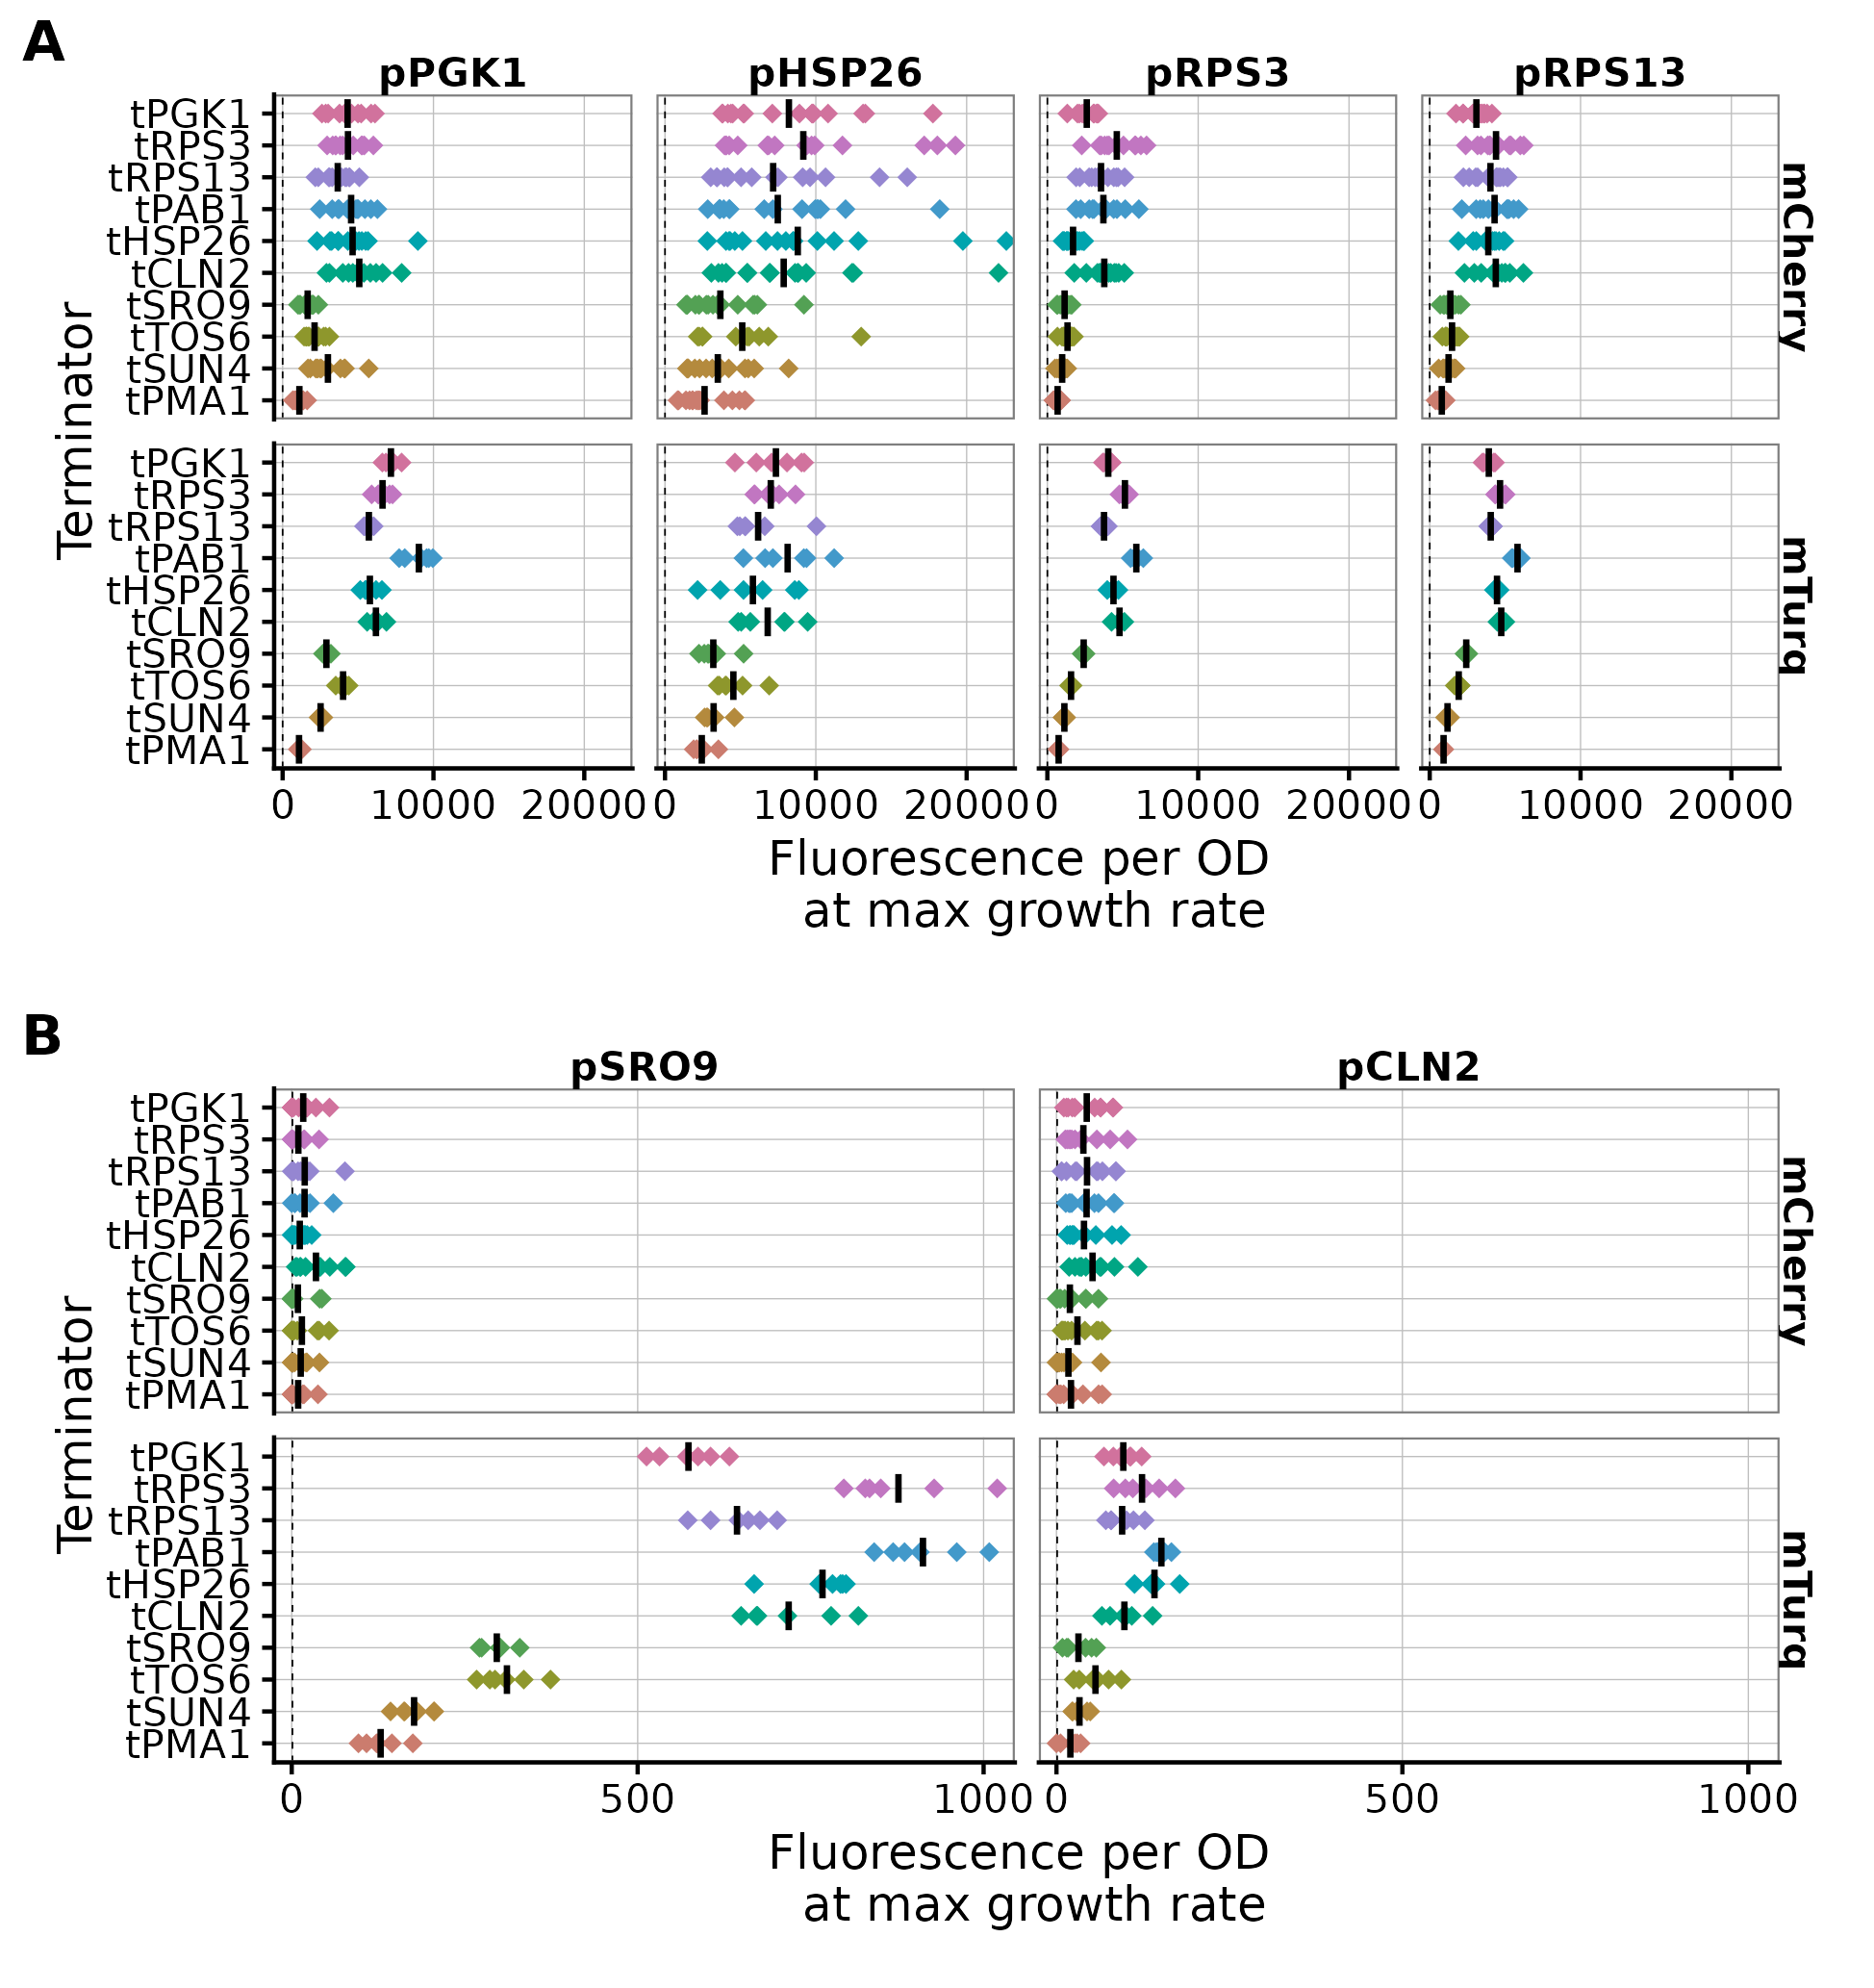
\includegraphics[width=\textwidth]{pro_ter_platereader_raw_mTurq_and_mCh} \caption[Both terminator and promoter contribute to gene expression.]{\textbf{Both terminator and promoter contribute to gene expression.} (\textbf{A}) Protein abundance estimated by mCherry and mTurquoise2 (mTurq) fluorescence for 10 terminators paired with 4 high expressing promoters. Fluorescence and OD were measured in cultures grown in a plate reader and reported at the time of the maximum growth rate of each sample (see methods). Each diamond represents a biological replicate, averaged over 3 technical replicates.  The vertical line is the mean of all 6 biological replicates. (\textbf{B}) Same as panel B, but for 2 low expressing promoters. Negative fluorescence values arising from instrument noise dominating measurements of constructs with negligible fluorescence are automatically set to 0.}\label{fig:raw-pro-ter-swap-protein-fluo}
\end{figure}

\begin{figure}[ph!]

{\centering 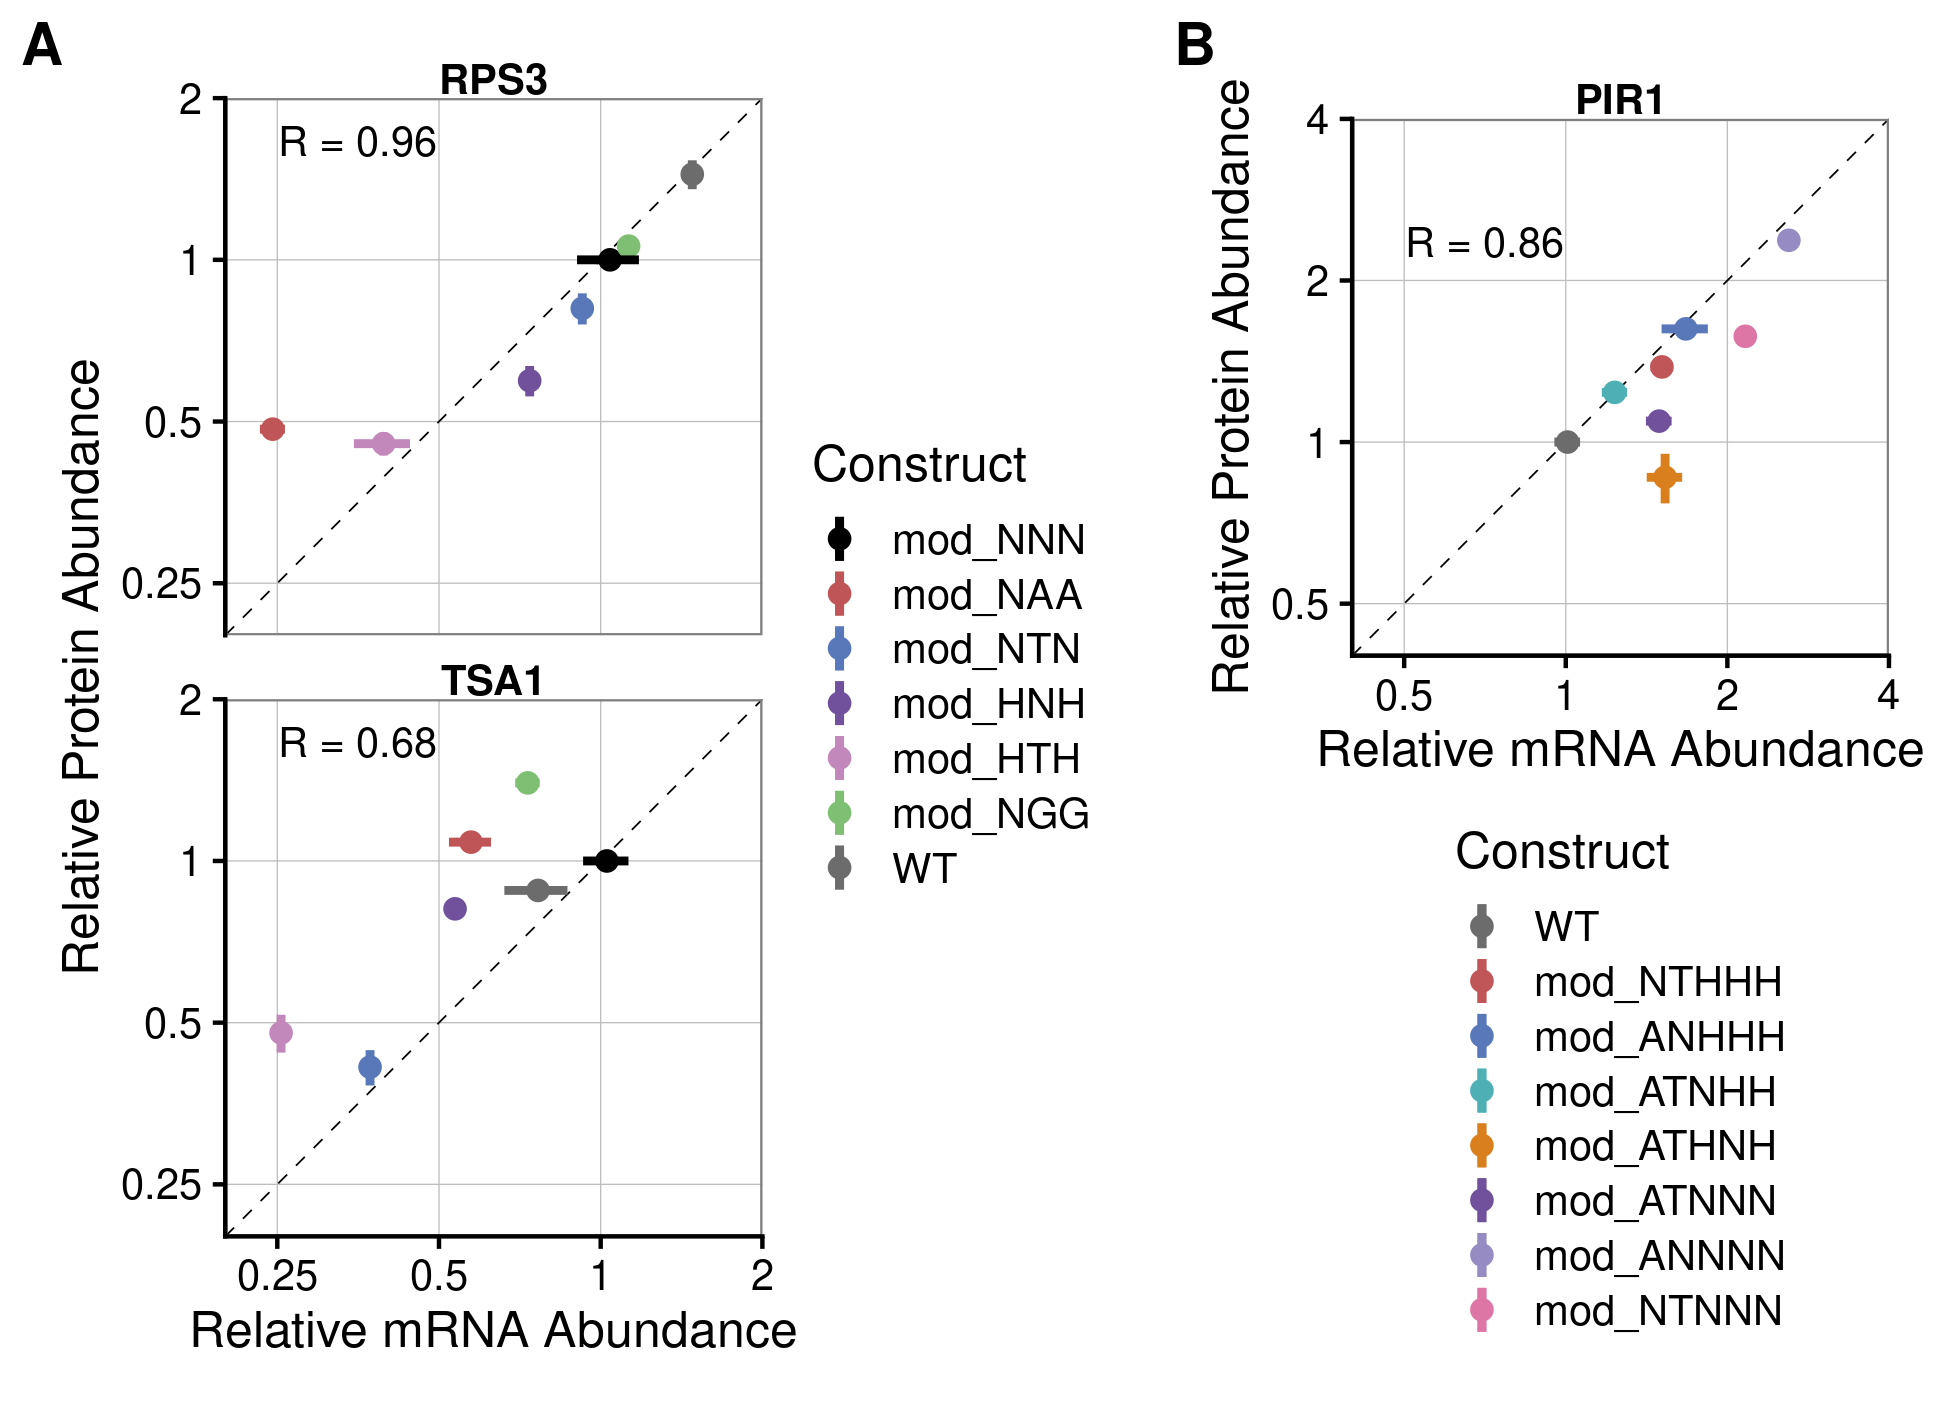
\includegraphics[width=0.98\linewidth]{RPS3_TSA1_PIR1_protein_and_RNA_plot} 

}

\caption[Relative protein abundance correlates with relative mRNA abundance for reporter constructs with modified 3'UTRs.]{\textbf{Relative protein abundance correlates with relative mRNA abundance for reporter constructs with modified 3'UTRs.} (\textbf{A}) Fold changes in RT-qPCR vs fold changes in mCherry fluorescence for all terminator constructs in the pRPS3-mCherry-tRPS3 and pTSA1-mCherry-tTSA1 pairings. Transcript abundance is relative to the mod0 construct of each promoter-terminator pairing. (\textbf{B}) Fold changes in RT-qPCR vs fold changes in mCherry fluorescence for all terminator constructs in the pPIR1-mCherry-tPIR1 pairing. Transcript abundance is relative to WT construct of the promoter-terminator pairing. The mean and standard error calculated over 6 biological replicates are plotted for each construct.}\label{fig:protein-vs-RNA-plot-motifs}
\end{figure}

\begin{figure}[ph!]

{\centering 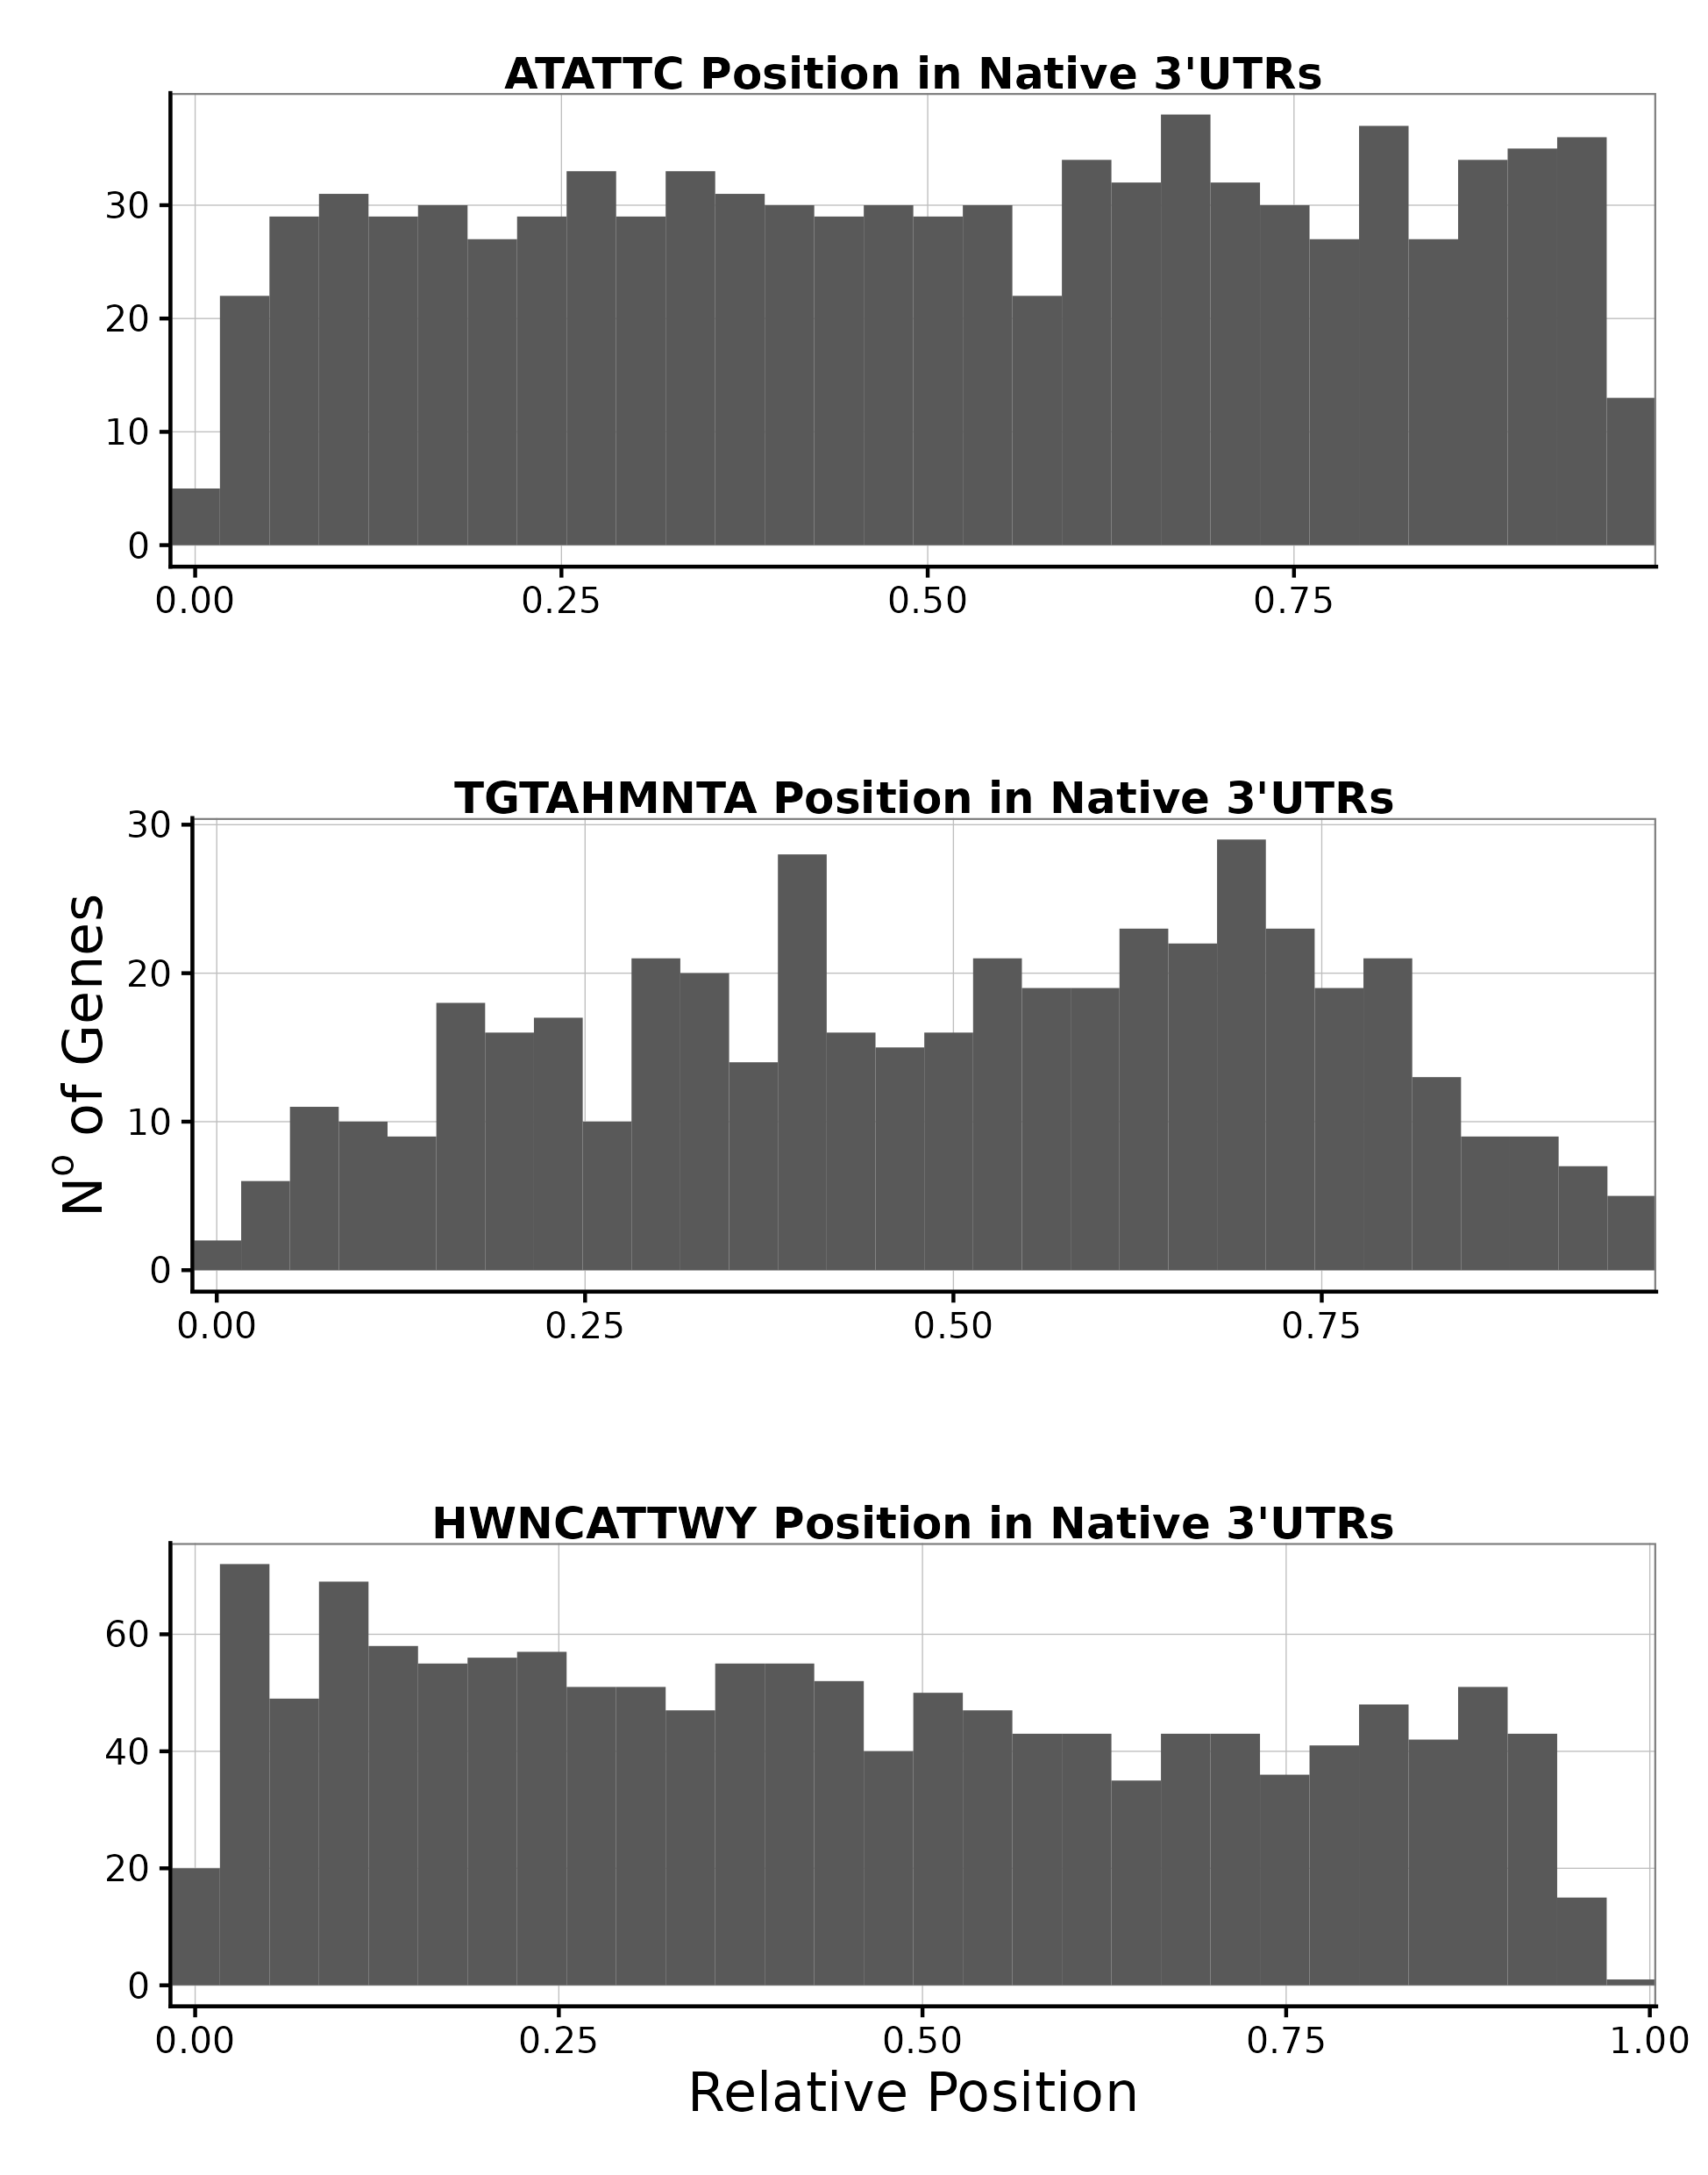
\includegraphics[width=0.98\linewidth]{motif_position_histograms} 

}

\caption[Relative positions of ATATTC, TGTAHMNTA and HWNCATTWY motifs in native 3'UTRs.]{\textbf{Relative positions of ATATTC, TGTAHMNTA and HWNCATTWY motifs in native 3'UTRs.} Histogram shows the counts of the motif occurrences in 3'UTRs relative to the total length of 3'UTR, where 0 would be starting exactly at the stop codon and 1 would be at the reported poly(A)-site. See (methods or ref to data repository) for details.}\label{fig:motif-position-histograms}
\end{figure}

\begin{figure}[ph!]

{\centering 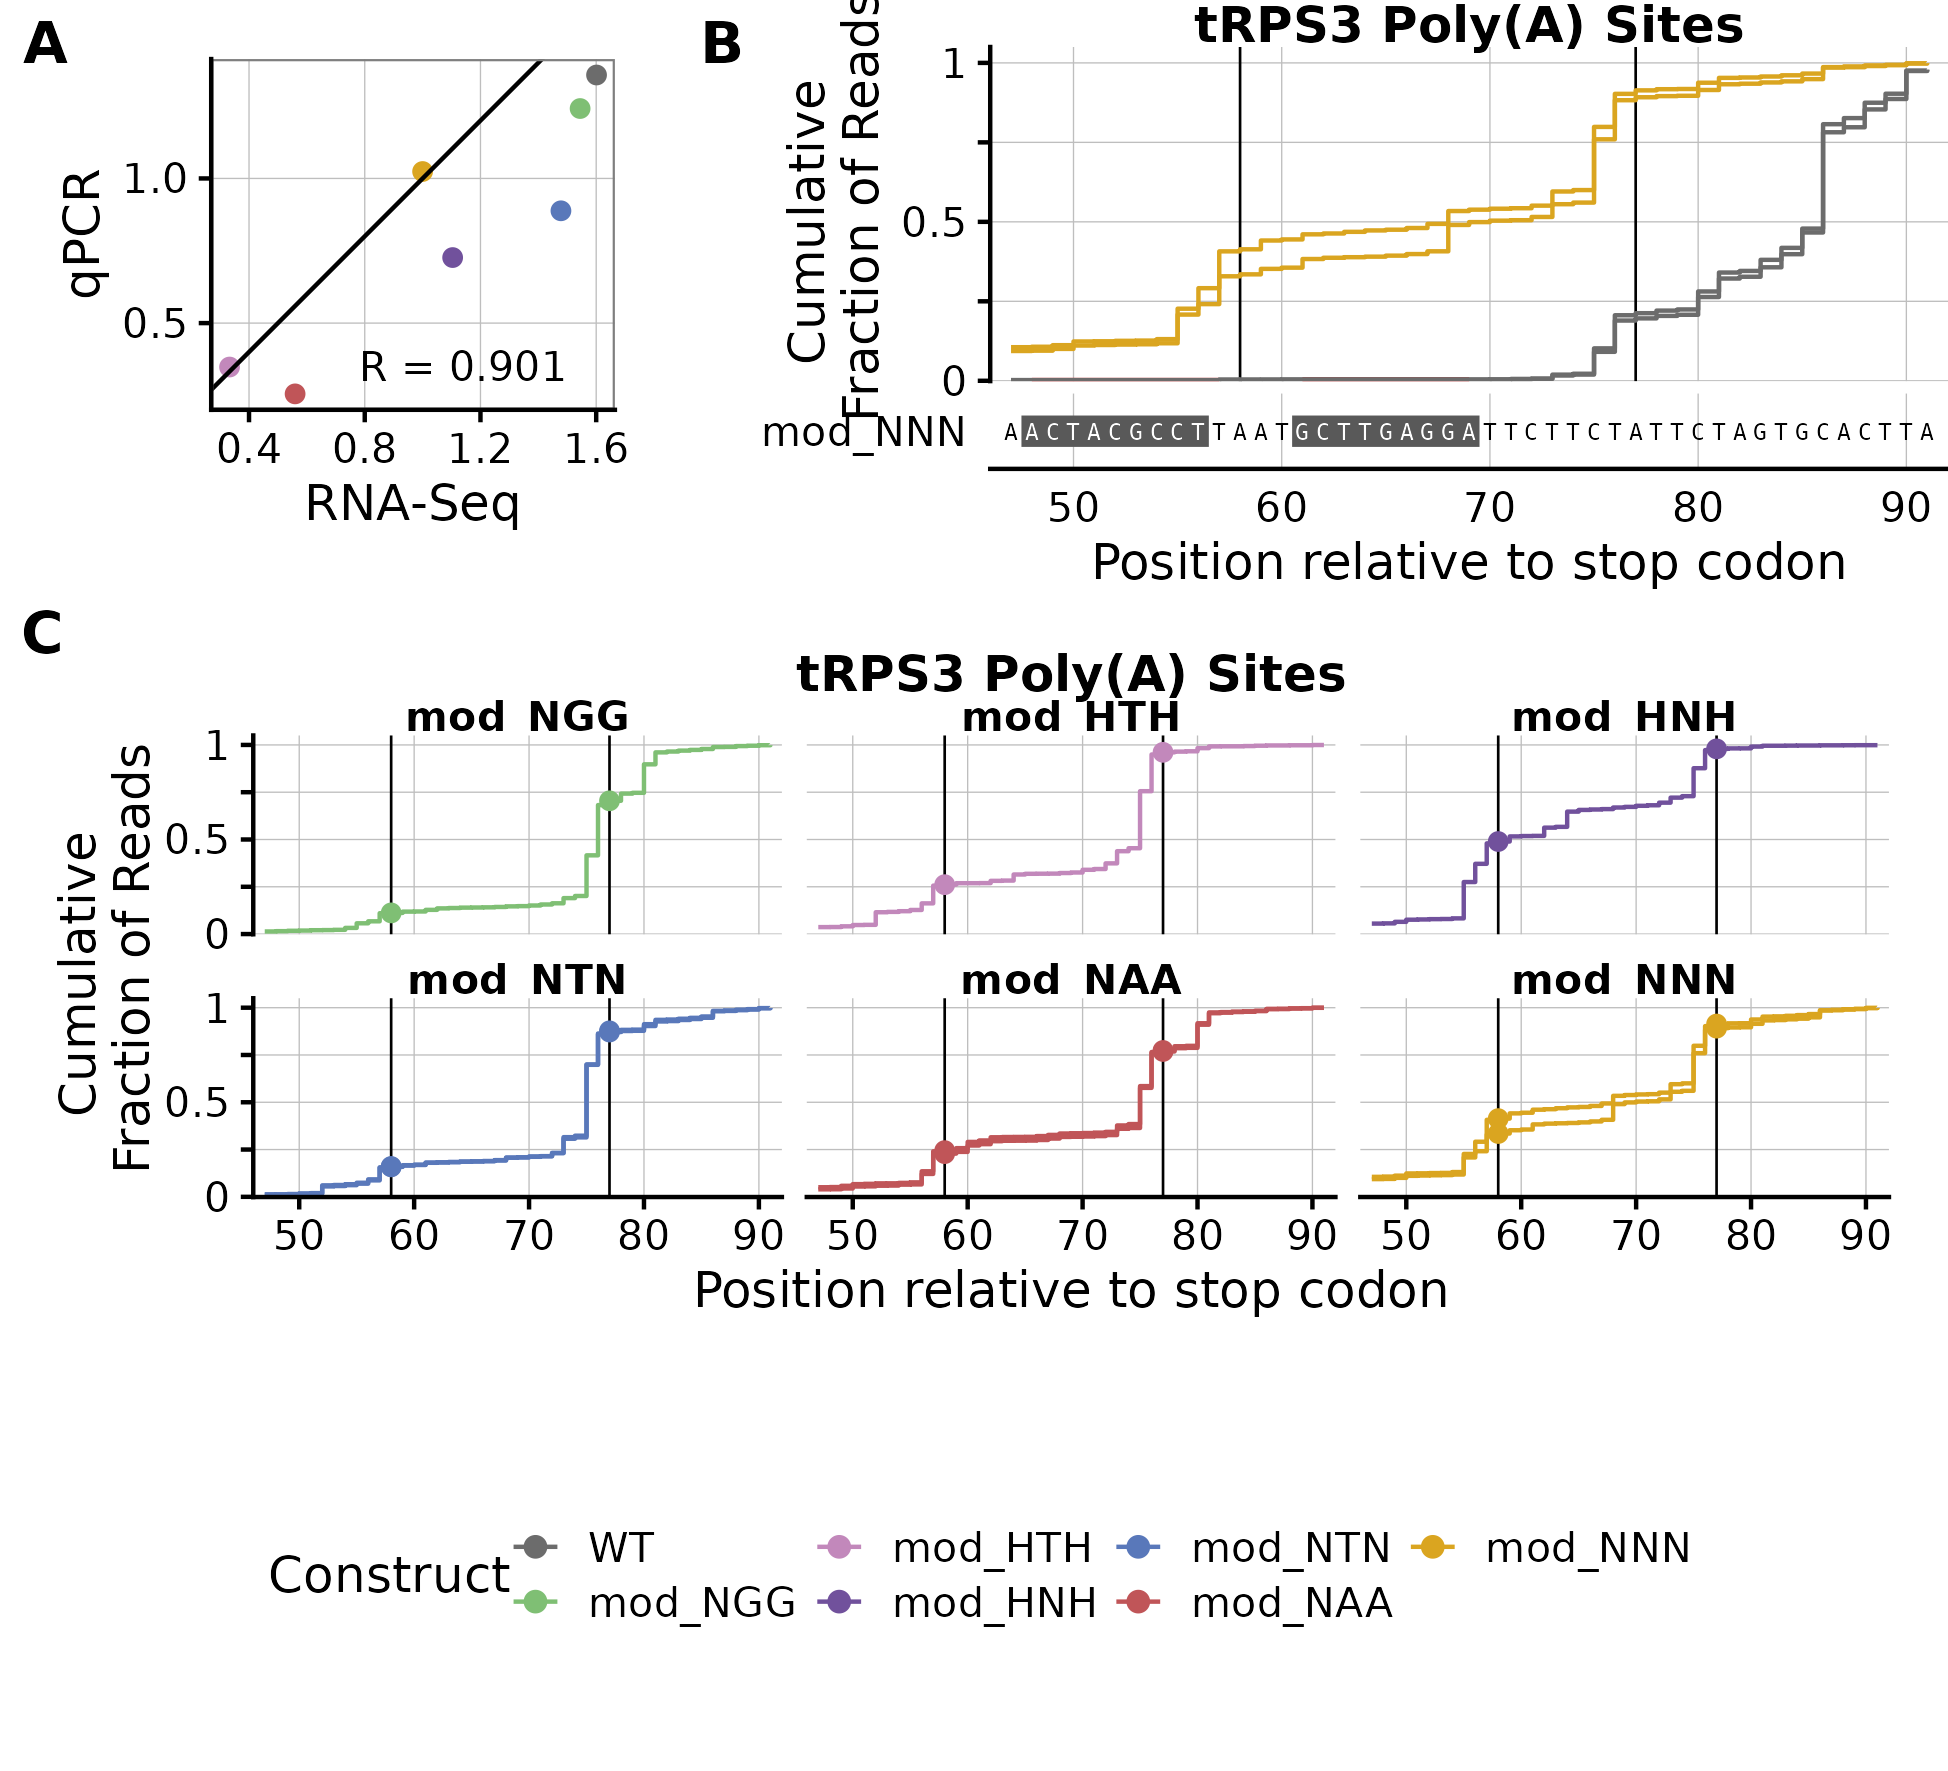
\includegraphics[width=0.85\linewidth]{polya_usage_plot_5PSeq} 

}

\caption[Decapped constructs measured by 5Pseq match mature constructs measured by QuantSeq.]{\textbf{Decapped constructs measured by 5Pseq match mature constructs measured by QuantSeq.} pRPS3-tRPS3 constructs were chosen to investigate changes in poly(A) site usage across 5' decapped transcripts flagged for decay. (\textbf{A}) Comparison of construct transcript abundance as independently measured by qPCR and RNA-Seq assays. Transcript abundance was normalised to the median abundance of  plasmid URA3, genomic PGK1 and RPS3 transcripts for each construct. Fold change is relative to the mod\_NNN construct in each promoter-terminator context. The black diagonal line represents the expected values of RNAseq and qPCR results correlated perfectly. (\textbf{B}) Cumulative counts of reads mapped downstream of WT (grey) and mod\_NNN (golden) construct stop codons as a fraction of the total reads mapped to the constructs terminator. WT reads have been shifted downstream to align with the mod\_NNN sequence by accounting for motif insertion sites. Major poly(A) sites have been highlighted by a black vertical line. Constructs also used in the QuantSeq analysis have their QuantSeq cumulative graphs plotted in dotted lines. (\textbf{C}) Similar to Figure \textbf{B} but with each motif insertion construct plotted separately. Columns designate cumulative plots from different terminator constructs.}\label{fig:polyA-site-usage-5Pseq}
\end{figure}

\begin{figure}[ph!]

{\centering 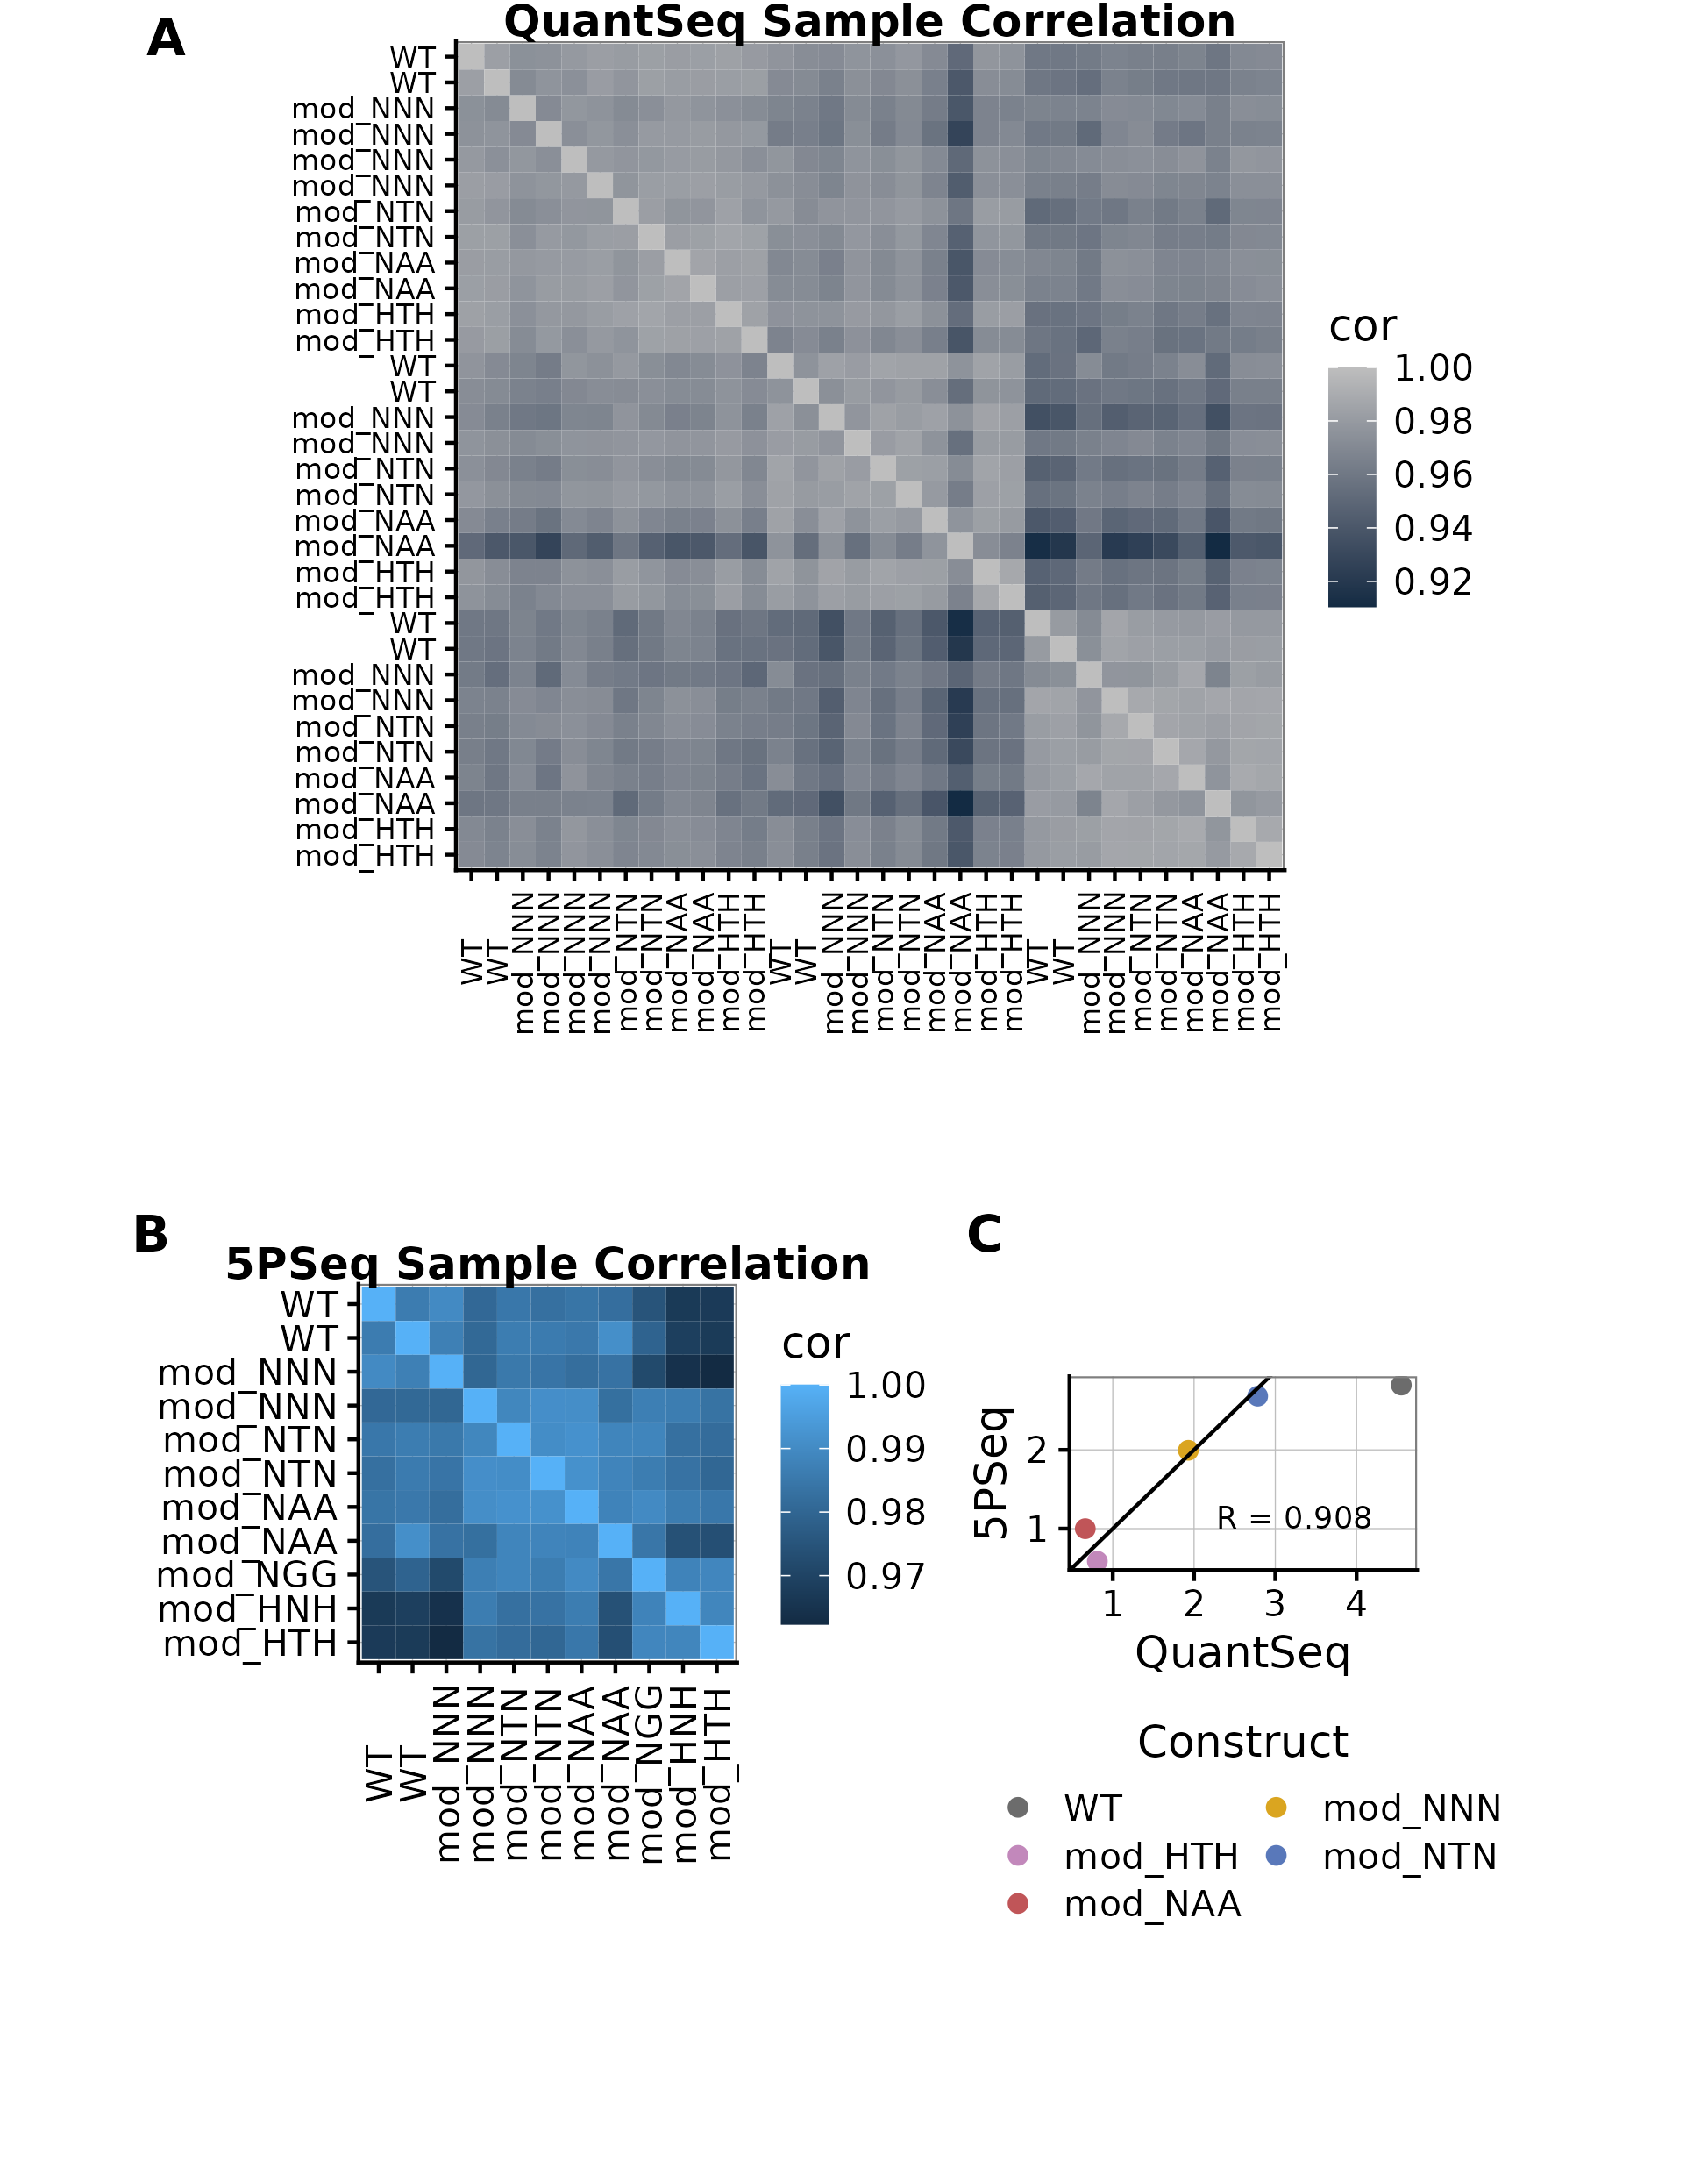
\includegraphics[width=0.85\linewidth]{sequencing_sample_correlation} 

}

\caption[High correlation in transcript counts between samples for both RNA-Seq assays.]{\textbf{High correlation in transcript counts between samples for both RNA-Seq assays.} (\textbf{A}) Correlation heat map of DESeq2 normalised log2 pseudocounts across all genes for each sample pair in the QuantSeq assay. From top to bottom on the y-axis (left to right on the x-axis) the terminator contexts are pRPS3-tRPS3, pPGK1-tRPS3 and pTSA1-tTSA1. (\textbf{B}) Similar correlation heat map for all sample pairs in the 5PSeq assay. (\textbf{C}) Comparison of mean log2 abundance of construct mRNA transcripts as measured by 5PSeq and QuantSeq. Only 5 terminator constructs were measured by both methods and only in the pRPS3-tRPS3 context. Transcript abundance for each sample is normalised to the median of the genomic PGK1, TSA1 and RPS3, and the plasmid URA3 genes to match the normalisation used in the qPCR analysis.}\label{fig:rnaseq-QC-correlation}
\end{figure}

\begin{figure}[ph!]

{\centering 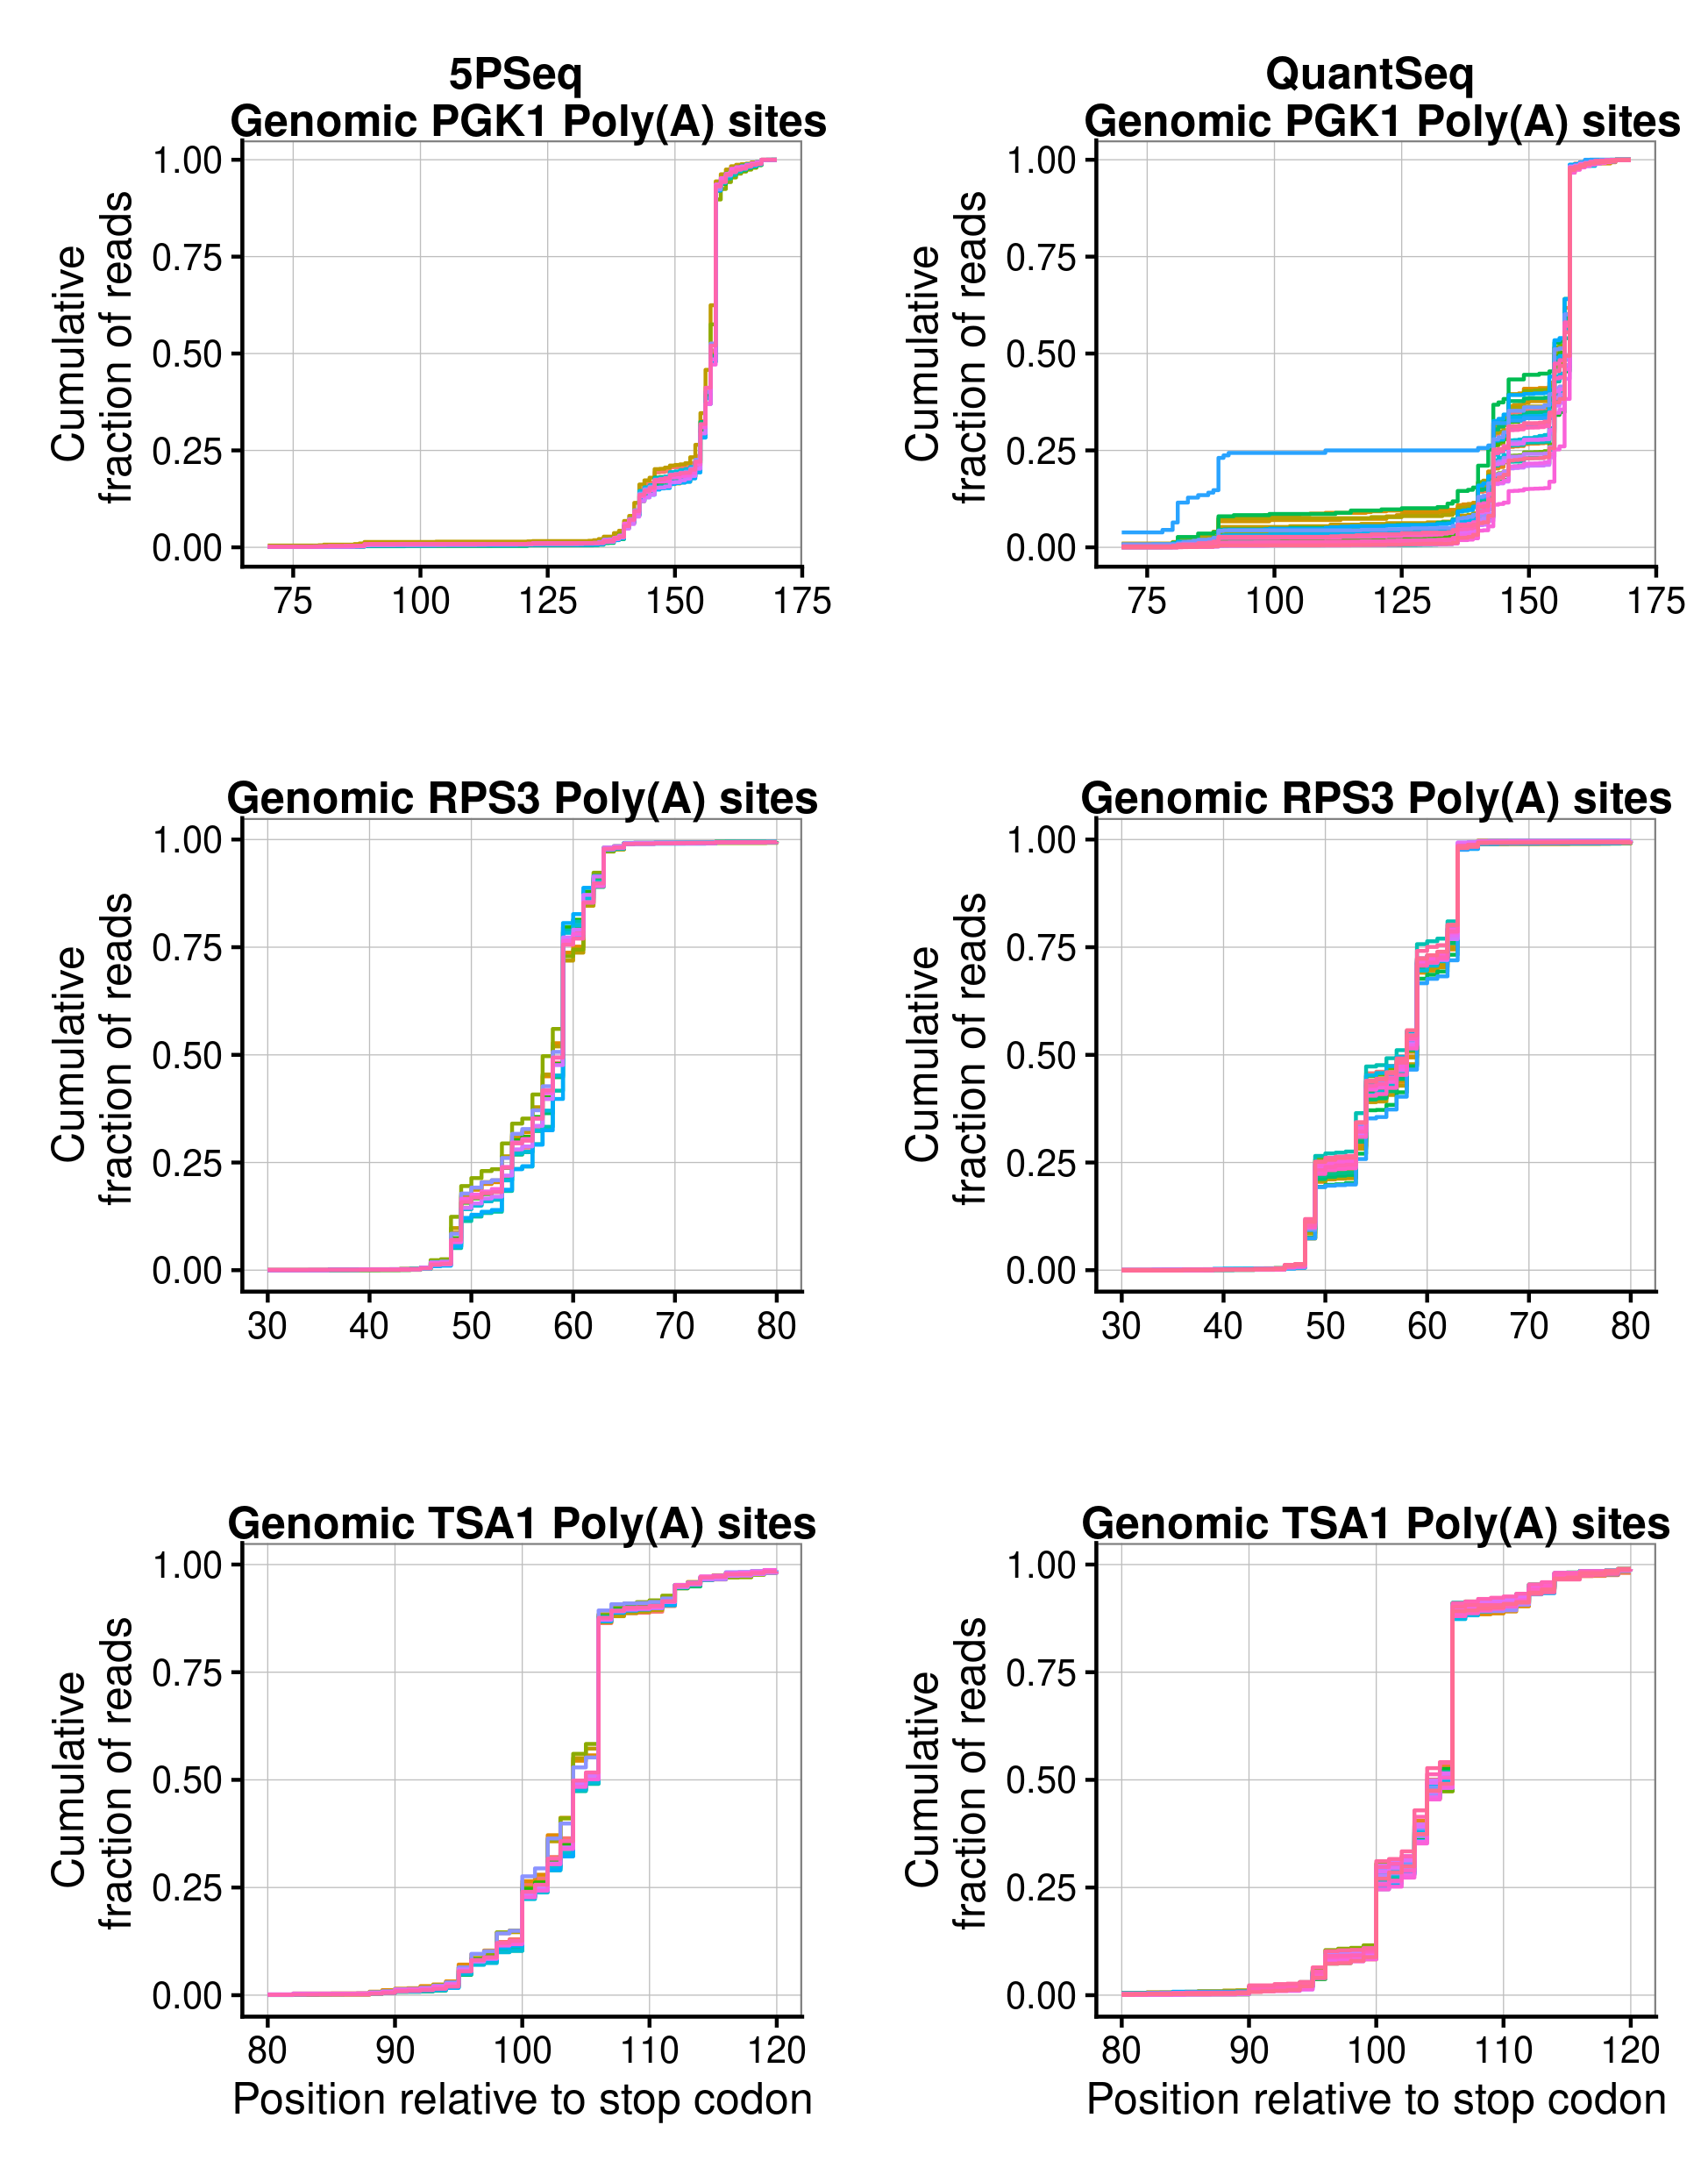
\includegraphics[width=0.85\linewidth]{polya_QC_plot_QuantSeq_and_5PSeq} 

}

\caption[Poly(A) site usage for genomic PGK1, TSA1 and RPS3 terminators remains the same across samples for each RNA-Seq assay.]{\textbf{Poly(A) site usage for genomic PGK1, TSA1 and RPS3 terminators remains the same across samples for each RNA-Seq assay.} Cumulative counts of reads mapped downstream of native genomic gene stop codons as a fraction of the total reads mapped to the terminator. Each line plots the cumulative counts of a separate sequencing run (including two tech reps per sample) which is given a unique colour. Relative usage of poly(A) sites remains similar across samples and across RNA-seq assays. Higher variability in QuantSeq PGK1 poly(A) site usage is due to low overall transcript counts.}\label{fig:rnaseq-QC-QuantSeq-and-5PSeq-genomic-polyA}
\end{figure}

\begin{figure}[ph!]

{\centering 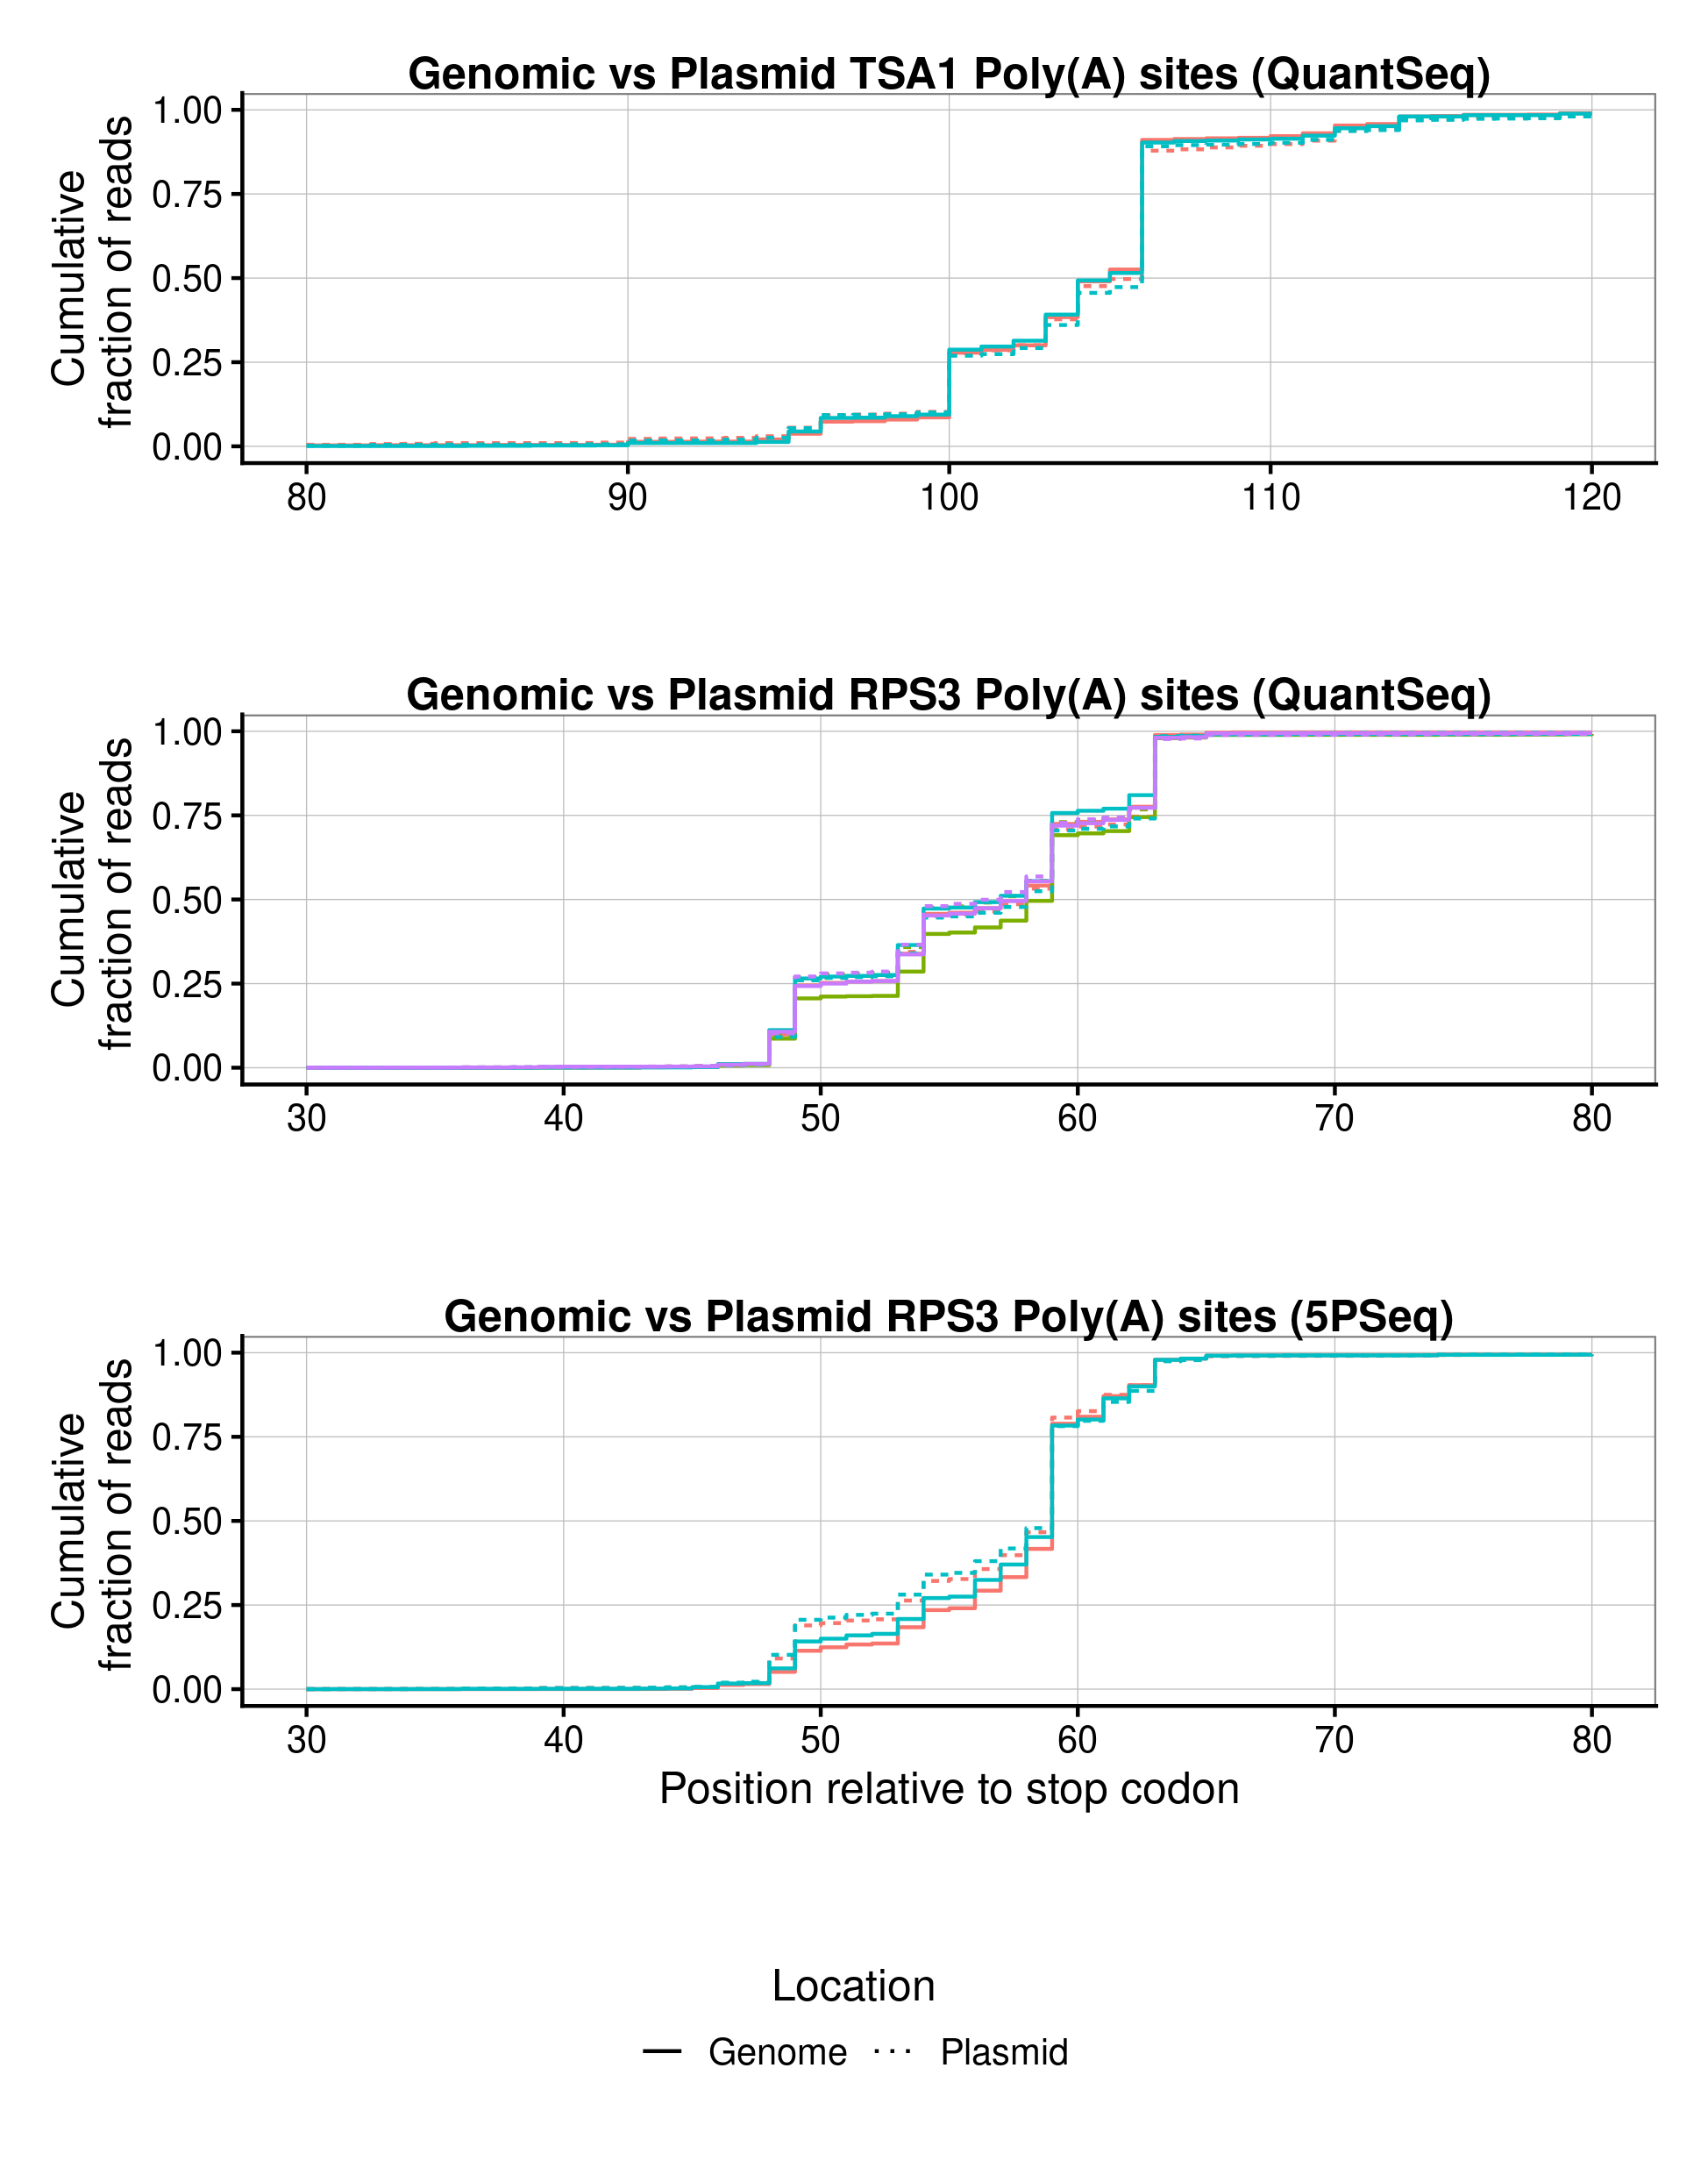
\includegraphics[width=0.85\linewidth]{plasmid_vs_genome_polyA_combined_plot} 

}

\caption[Poly(A) site usage remains the same for genomic TSA1 and RPS3 terminators as for plasmid expressed WT constructs in QuantSeq and 5PSeq.]{\textbf{Poly(A) site usage remains the same for genomic TSA1 and RPS3 terminators as for plasmid expressed WT constructs in QuantSeq and 5PSeq.} Cumulative counts of reads mapped downstream of WT stop codons for native genomic terminators and plasmid construct terminators as a fraction of total reads mapped to the constructs terminator. Each line plots the cumulative counts of a separate sequencing run (including two tech reps per sample) which is given a unique colour. Expressing constructs from a low copy number plasmid does not seem to affect poly(A) site usage.}\label{fig:rnaseq-QC-genomic-vs-plasmid-polyA}
\end{figure}

\begin{figure}[p]

{\centering 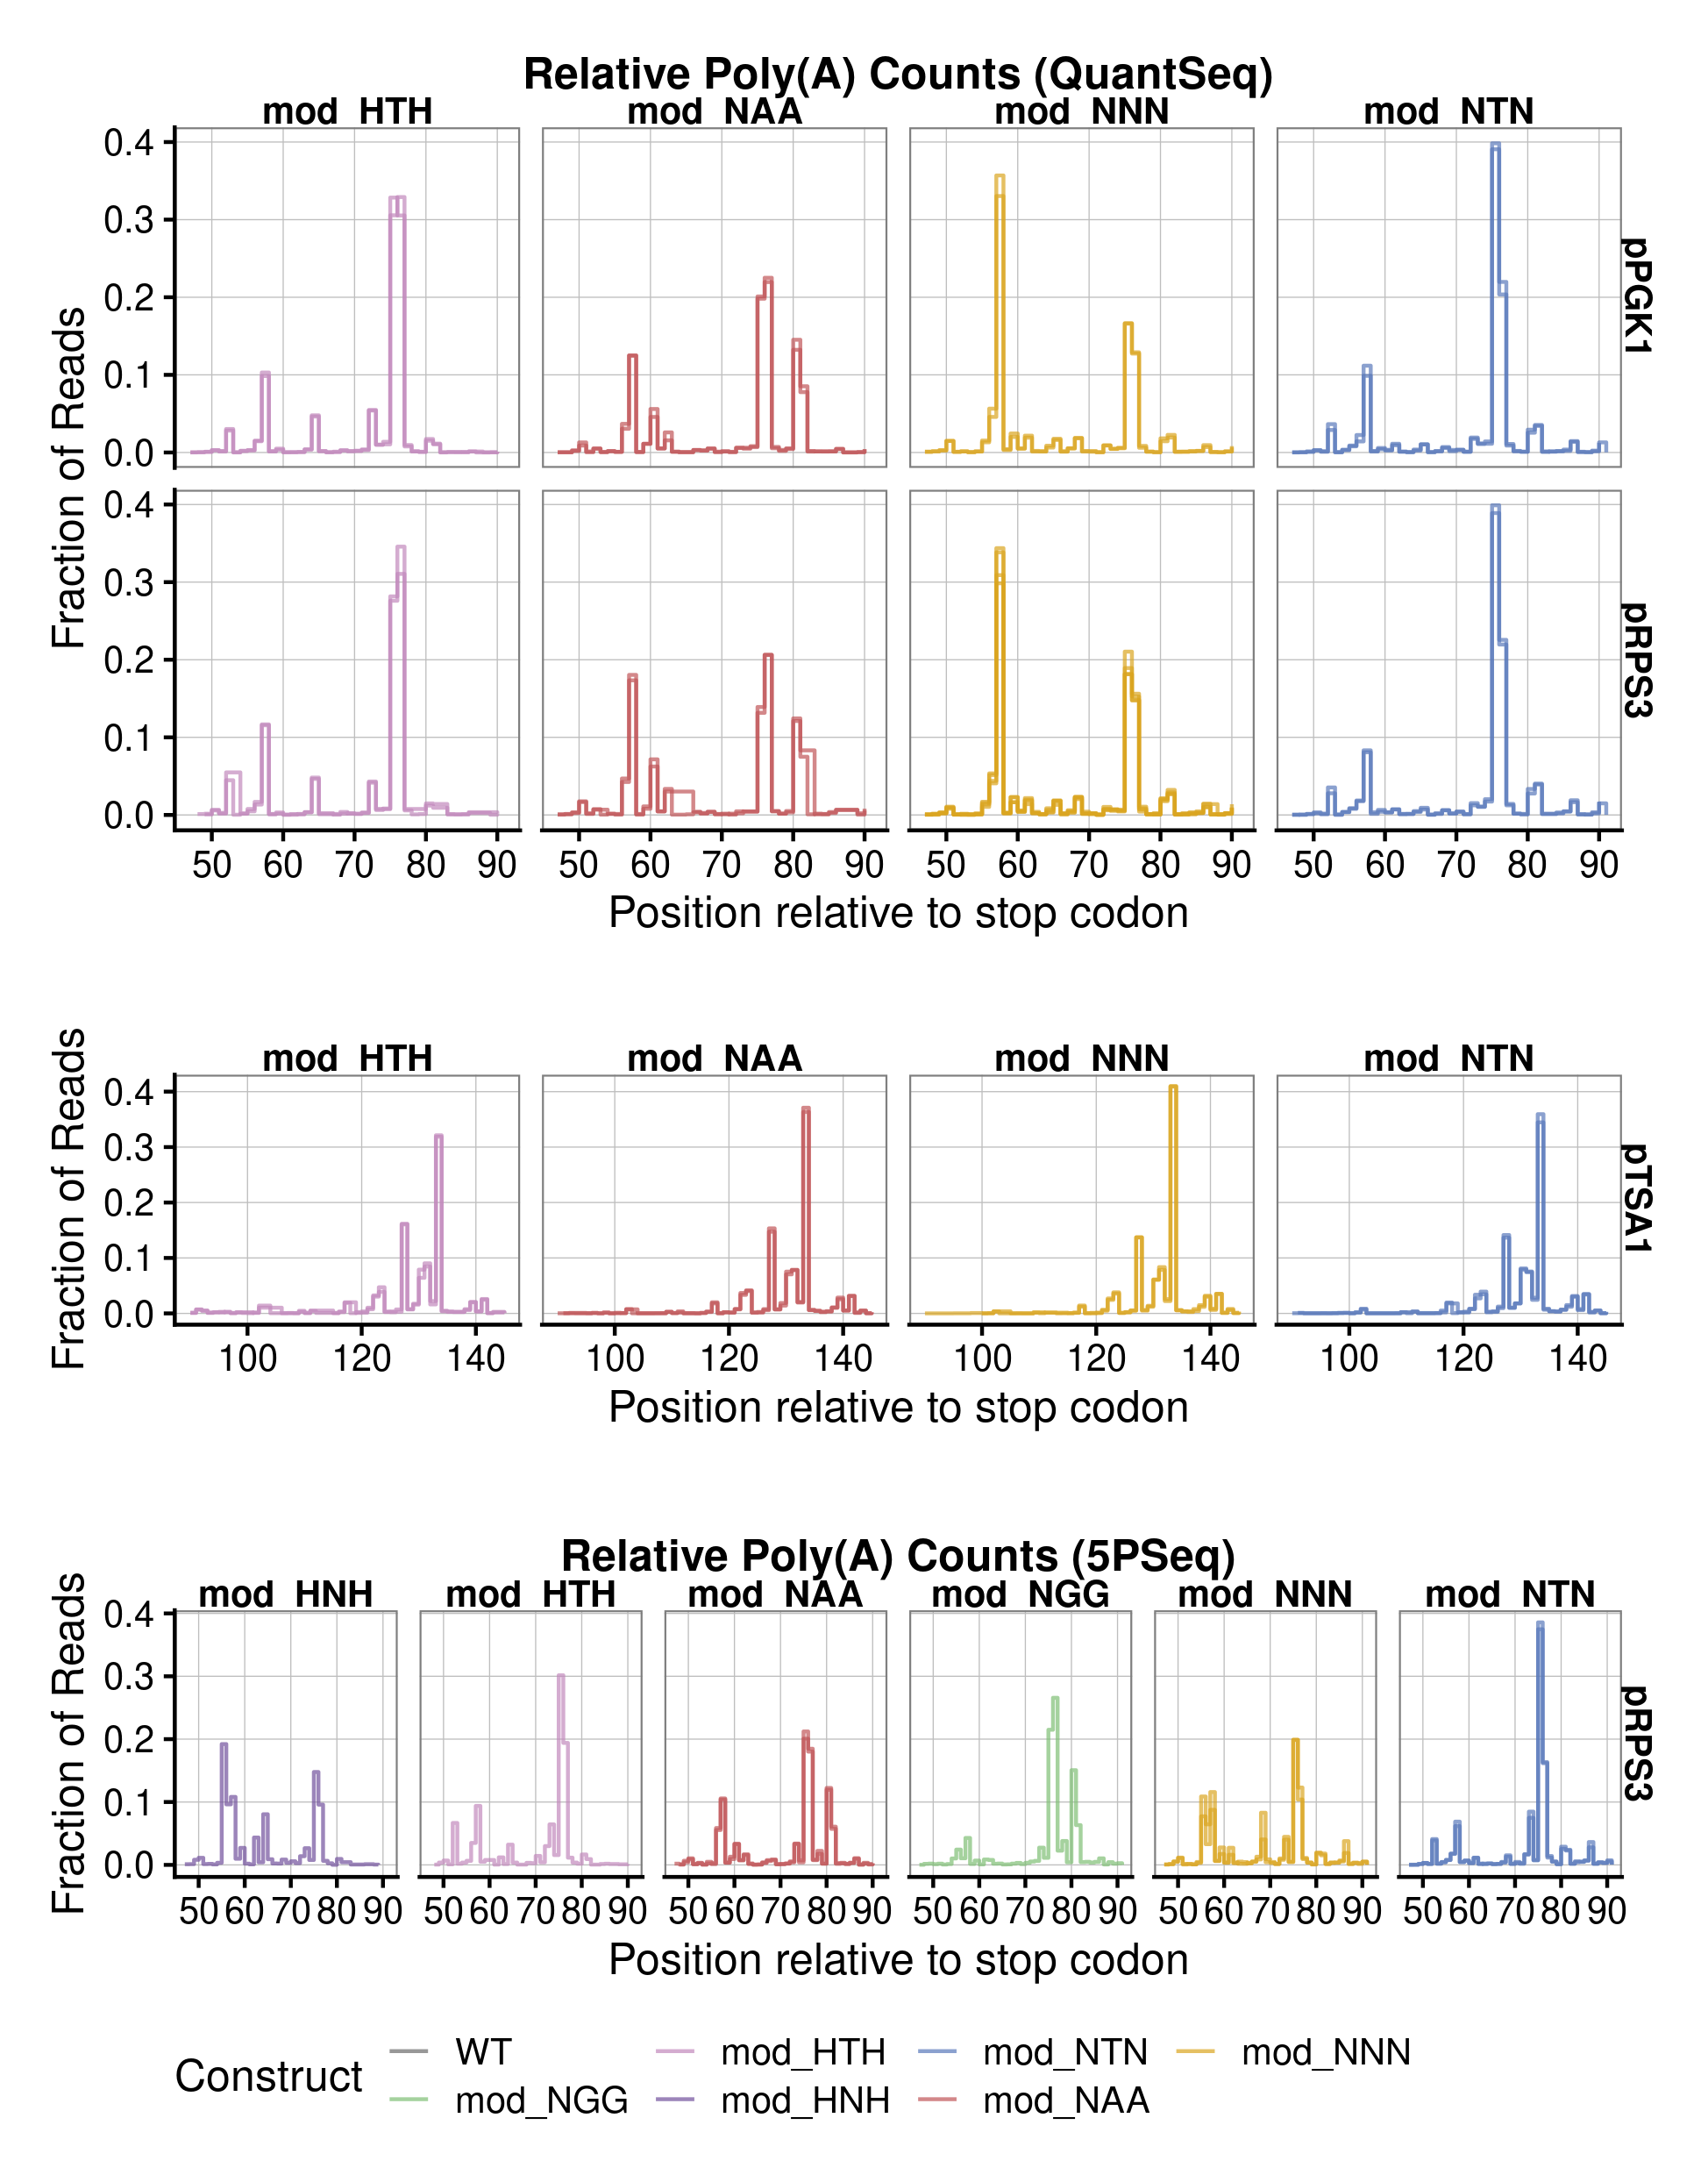
\includegraphics[width=0.85\linewidth]{relative_polya_counts_QuantSeq_and_5PSeq} 

}

\caption[Construct poly(A) site usage across 5PSeq and QuantSeq.]{\textbf{Construct poly(A) site usage across 5PSeq and QuantSeq.} Relative counts of reads mapped downstream of construct stop codons as a fraction of the total reads mapped to the constructs terminator. Peaks represent the position of major poly(A) sites. Replicates are plotted on top of each other where available.}\label{fig:relative-polya-counts}
\end{figure}

\begin{figure}[ph!]

{\centering 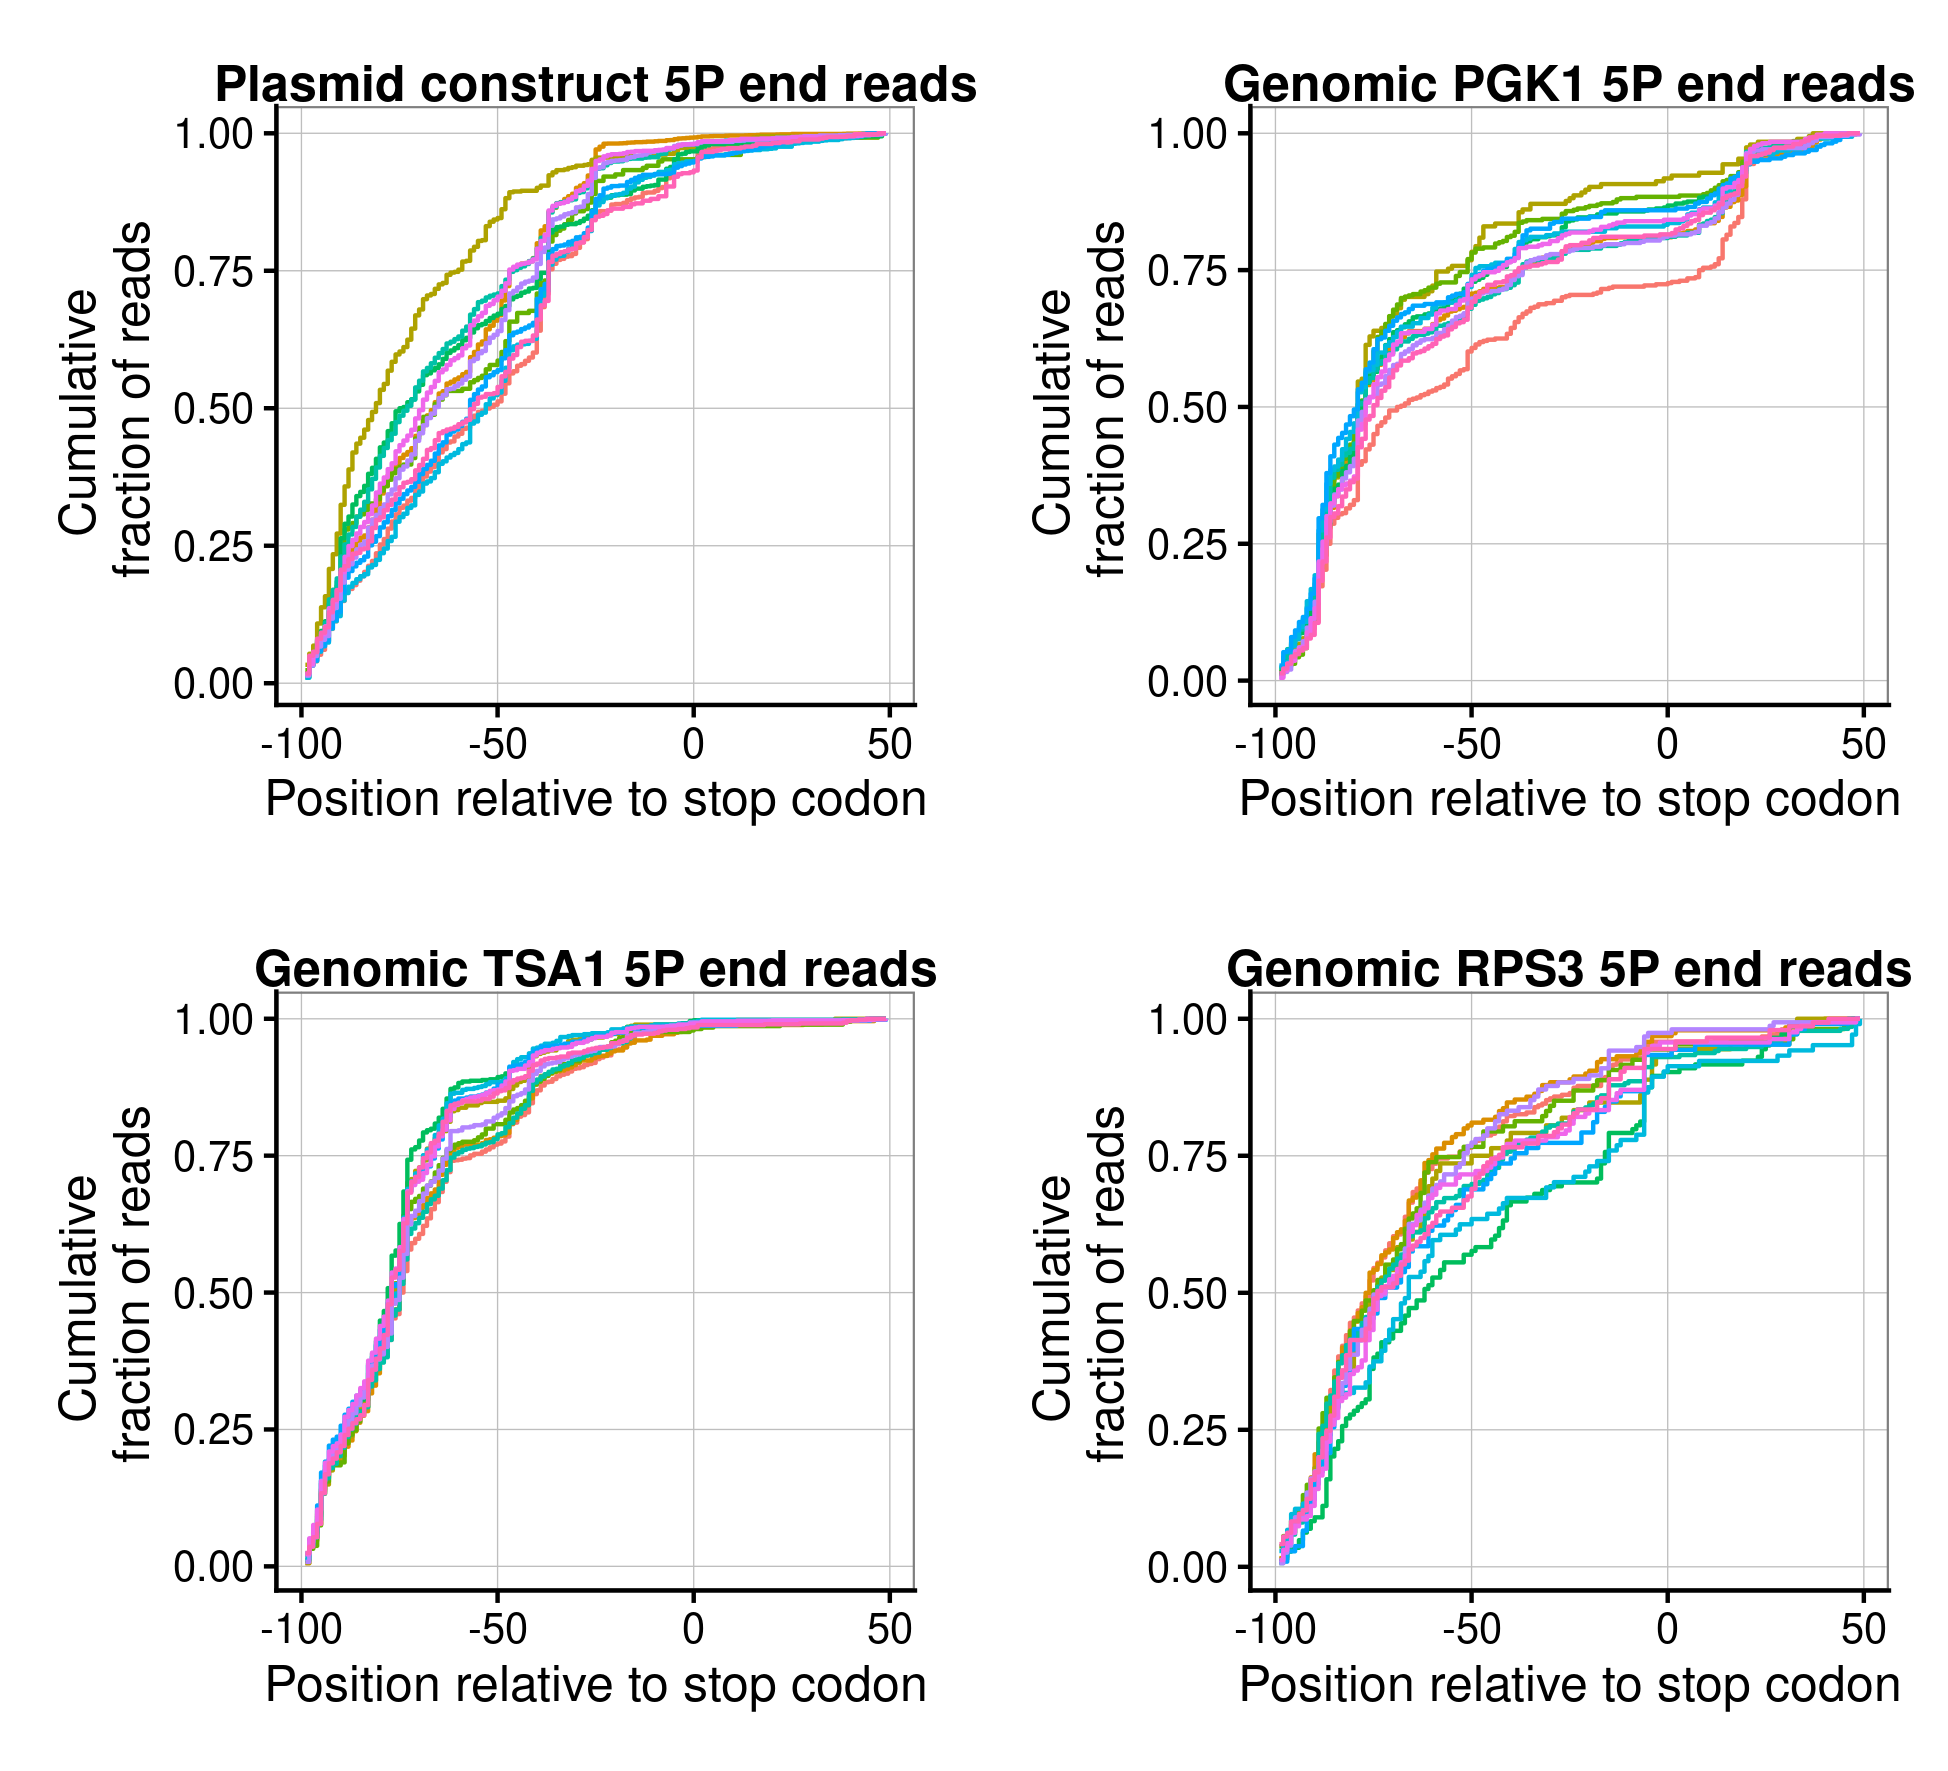
\includegraphics[width=0.85\linewidth]{combined_5p_end_read_plot} 

}

\caption[5PSeq data finds no detectable changes in 5'-phosphorylated intermediates between reporter constructs.]{\textbf{5PSeq data finds no detectable changes in 5'-phosphorylated intermediates between reporter constructs.} Relative counts of 5' end reads of 5'-phosphorylated intermediates as a fraction of the total 5' end reads mapped to the terminator. Results for plasmid constructs are plotted alongside selected genomic genes for comparison.}\label{fig:combined-5p-end-read-plot}
\end{figure}

\end{document}